
\documentclass[10pt,a4paper,oneside,openright,%
               parskip=half,%
               BCOR=5mm,DIV=10,footinclude=false%
               numbers=noenddot,cleardoublepage=empty]{scrbook}

\usepackage[utf8]{inputenc} 
\usepackage[sc]{mathpazo} %-- use Palatino font
\usepackage{amsmath,amssymb,amsthm}
\usepackage{natbib}
\usepackage{xspace}
\usepackage[breaklinks=true,
            colorlinks=true,
            linktocpage=true,
            allcolors=colorforlinks]{hyperref} 
\usepackage[capitalise]{cleveref}
\usepackage[ruled,vlined,algochapter,linesnumbered]{algorithm2e}
\usepackage{calc}
\usepackage{ccicons} 
\usepackage{xspace} 
\usepackage{tabularx}
\usepackage{booktabs} 
\usepackage[english]{babel}  
\usepackage{listings}
\usepackage{scrhack} % ignore warnings about deprecated KOMA-Script
\usepackage[printonlyused,smaller,withpage]{acronym}
\usepackage[usenames,dvipsnames]{xcolor}
\usepackage{graphicx}
\usepackage{pdfpages}
\usepackage{todonotes}
\usepackage{footnote}
\usepackage{enumitem}
\usepackage{multirow}
\usepackage{float}
\usepackage{graphicx,subfigure}

% \setlength{\abovecaptionskip}{15pt plus 3pt minus 2pt}
\setlength\abovecaptionskip{\baselineskip}
\setlength\belowcaptionskip{\baselineskip}

\graphicspath{ {./resources/} }

\newcolumntype{R}[1]{>{\raggedleft\arraybackslash}p{#1}}
\newcolumntype{L}[1]{>{\raggedright\arraybackslash}p{#1}}
\newcolumntype{C}[1]{>{\centering\arraybackslash}m{#1}}

\providecommand\algorithmname{algorithm}

\crefname{line}{line}{lines}

\newcommand{\mathbfcal}[1]{\pmb{\mathcal{#1}}}

\theoremstyle{definition}
\newtheorem{secDefinition}{Definition}[section]



\newcommand{\myName}{
    Egor Dmitriev (6100120) \\
    egordmitriev2@gmail.com
}
\newcommand{\myTitle}{MGTCOM: Community Detection in Temporal Multimodal Graphs}

\newcommand{\myUni}{Utrecht University}

\newcommand{\myGraduationYear}{2022}
\newcommand{\myGraduationMonth}{June}

\newcommand{\mySupervisorOne}{Dr. M. W. Chekol}
\newcommand{\mySupervisorTwo}{Dr. S. Wang}

%-- for names for \autoref commands
\def\chapterautorefname{Chapter}
\def\sectionautorefname{Section}
\def\subsectionautorefname{Section}
\def\subsubsectionautorefname{Section}
\def\algorithmautorefname{Algorithm}
 
%-- for pdf metadata
\hypersetup{pdfauthor={\myName}}
\hypersetup{pdfkeywords={community detection, representation learning, dynamic networks}}
\hypersetup{pdfsubject={A thesis submitted to the Utrecht University in partial fulfillment of the requirements for the degree of Master of Science in Computing Science}}
\hypersetup{pdftitle={\myTitle}}

%-- handy shortcuts
\newcommand{\ie}{i.e.}
\newcommand{\eg}{e.g.}

%-- colours for the hyperlinks
\definecolor{colorforlinks}{RGB}{27, 60, 131}




\setcapindent{1em} %-- for captions of Figures
% \setcounter{tocdepth}{\sectiontocdepth}

\subject{MSc thesis in Computing Science}
\title{\myTitle}
\author{\myName}
\date{\myGraduationMonth\xspace\myGraduationYear}
\publishers{
    \noindent
    \large
    \textbf{Supervisors} \\
    \vspace{1mm}
    \begin{tabular}{lll}
    \mySupervisorOne & m.w.chekol@uu.nl & Utrecht University \\
    \mySupervisorTwo & s.wang2@uu.nl & Utrecht University \\
    \end{tabular}
    
    \vspace{12mm}
    A thesis submitted to the Utrecht University in partial fulfillment of the requirements for the degree of Master of Science in Computing Science
    
    \vspace{12mm}
    
\includegraphics[width=0.4\textwidth]{resources/uu.png}
}

\begin{document}


%******************************************************************
% Frontmatter
%******************************************************************
\frontmatter

% \includepdf{cover/cover_front.pdf}
% \cleardoublepage

\maketitle[3]

% \clearpage
\cleardoublepage

\chapter*{Abstract}
Community detection is the task of discovering groups of nodes sharing similar patterns within a network.
With recent advancements in deep learning, methods utilizing graph representation learning and deep clustering have shown great results in community detection.
However, these methods often rely on the topology of networks (i) ignoring important features such as network heterogeneity, temporality, multimodality and other possibly relevant features.
Besides, (ii) the number of communities is not known a priori and is often left to model selection.
In addition, (iii) in multimodal networks all nodes are assumed to be symmetrical in their features; while true for homogeneous networks, most of the real-world networks are heterogeneous where feature availability varies.
In this paper, we propose a novel framework (named MGTCOM) that overcomes the above challenges (i)--(iii). MGTCOM allows to discover dynamic communities through multimodal feature learning by leveraging a new sampling technique for unsupervised learning of temporal embeddings. Importantly, MGTCOM is an end-to-end framework optimizing network embeddings, communities, and the number of communities in tandem.
In order to assess its performance, we carried out an extensive evaluation on a number of multimodal networks.
We found out that our method is competitive against state-of-the-art and performs well under the inductive setting.
% \chapter*{Acknowledgements}
\clearpage

\setcounter{tocdepth}{2}

\tableofcontents
\listoffigures
\listoftables
\listofalgorithms


\clearpage
% \chapter*{Acronyms}

% \begin{acronym}[UML]
%   \acro{dem}[DEM]{digital elevation model}
%   \acro{dt}[DT]{Delaunay triangulation}
%   \acro{gdal}[GDAL]{Geospatial Data Abstraction Library}
%   \acro{gis}[GIS]{geographical information system}
%   \acro{giss}[GISs]{geographical information systems}
%   \acro{gui}[GUI]{graphical user interface}
%   \acro{tin}[TIN]{triangular irregular network}
%   \acro{vd}[VD]{Voronoi diagram}
% \end{acronym}
\cleardoublepage

%******************************************************************
% Mainmatter
%******************************************************************
\mainmatter

\chapter{Introduction}

% Networks and Community Detection
Various systems can be modelled as complex networks such as 
social \cite{hagenCrisisCommunicationsAge2018}, citation \cite{mccallumAutomatingConstructionInternet2000, senCollectiveClassificationNetwork2008}, biological \cite{gosakNetworkScienceBiological2018} and transaction \cite{prykeAnalysingConstructionProject2004} networks.
The task of identifying patterns of nodes with common properties, in such networks, is referred to as community detection.
% 
There is an abundant number of community detection methods in literature that approach this problem through modularity optimization \cite{newmanFastAlgorithmDetecting2004, blondelFastUnfoldingCommunities2008, schuetzMultistepGreedyAlgorithm2008}, clique identification \cite{farkasWeightedNetworkModules2007, kumpulaSequentialAlgorithmFast2008}, and spectral optimization \cite{wangCommunityDiscoveryUsing2011, heLaplacianRegularizedGaussian2011}.
% Emergence of graph representation learning
With recent advancements in graph representation learning a new type of methods have emerged which 
utilize context-based learning techniques (e.g., DeepWalk \cite{perozziDeepWalkOnlineLearning2014}, LINE \cite{tangLINELargescaleInformation2015} or Node2Vec \cite{groverNode2vecScalableFeature2016}) to obtain topology-aware node embeddings.
These embeddings are either combined with existing clustering methods \cite{caoIncorporatingNetworkStructure2018, xueCrossdomainNetworkRepresentations2019}
or are jointly optimized with found clusters 
\cite{cavallariLearningCommunityEmbedding2017, rozemberczkiGEMSECGraphEmbedding2019, jiaCommunityGANCommunityDetection2019}
to obtain communities.

% Problem 1: Overlooked features
In the above studies, the dynamic and multimodal characteristics of real-world networks are overlooked. 
These characteristics can manifest as meta-topological features (node and relation types) \cite{caoKnowledgePreservingIncrementalSocial2021}, temporal features, and contentual features (e.g., text and image attributes).
%
Introduction of multimodality contrasts \textit{homophily} assumed by previous methods as \textit{heterophily} and can play an essential role in detecting communities in multimodal networks, as connected nodes may belong to different communities when multiple feature types are considered \cite{zhuHomophilyGraphNeural}.  
% 
While it is common for causal links to be present between these features, it cannot be assumed without extensive domain knowledge.
% 
Various algorithms have been devised to address the issue of temporality and multimodality \cite{greeneTrackingEvolutionCommunities2010, luoDetectingCommunitiesHeterogeneous2021, liCommunityDetectionAttributed2018, faniUserCommunityDetection2020}, 
though as far as we are aware none of the methods are able to address the lossless setting where all the features are incorporated.

% Problem 2: Information variance / asymmetry
Another challenge is information variance present in heterogeneous real-world networks. 
Different node or relation types may have different feature subsets and/or dimensionality.
% Example
Let us consider the Twitter dataset (SDS) we use as a case study in \cref{sec:case_study}. 
This network consists of users, tweets, hashtags, and various relations in-between. 
Here tweets have content as textual features and post dates as temporal features, while users only have biography as textual features, and hashtags have neither. 
Similarly, users form a directed follower relation link, while multiple relations may be present between tweets such as retweet, mention or quote.
The meta-topological information describes important semantics of this network, while varying features and topology can be used to identify individual nodes.
If these characteristics are ignored by a model, then the quality of the communities discovered can be affected. 

% Problem 3: Scale / Topologically incomplete networks
With the emergence of web-scale network datasets (often exceeding billions of nodes), recent advancements have pushed for scalability in graph representation learning \cite{hamiltonInductiveRepresentationLearning2017, yingGraphConvolutionalNeural2018}. 
To this end, graph convolution methods have allowed for inductive inference on unseen nodes no longer requiring storing full graph Laplacian or node embeddings in memory. 
Utilizing this representation function learning helps solve scaling issues faced by many auto-encoder-based and shallow embedding community detection methods \cite{mehtaStochasticBlockmodelsMeet2019, panAdversariallyRegularizedGraph2018, wangDynamicCommunityDetection2017a}.

% TODO: possibly create a list of all the challenges. An overview

In this paper, we propose a novel community detection framework (MGTCOM) that is able to address the aforementioned challenges.
MGTCOM discovers dynamic communities through multimodal feature learning and unsupervised learning with a new sampling technique. 
In particular, our key contributions include:
%
\begin{itemize}[leftmargin=*]
    \item[(i)] A robust method for unsupervised representation learning on multimodal networks
    \item[(ii)] A new sampling technique for unsupervised learning of temporal embeddings
    \item[(iii)] An end-to-end framework optimizing network embeddings, communities, and number of communities in tandem
    \item[(iv)] Extensive evaluation on the quality of various features in multimodal networks
    \item[(v)] Implementation of various graph sampling algorithms found in the literature\footnote{https://github.com/EgorDm/tch-geometric} (See \href{https://anaconda.org/egordm/tch_geometric}{repository}).
\end{itemize}
%
We compare MGTCOM with state-of-the-art methods and demonstrate its robustness on inference tasks.

The rest of the thesis is organized as follows. 
Related works and relevant material is discussed in \cref{sec:related_work} and \cref{sec:preliminaries} respectively.
\cref{sec:approach} covers the details of our frameworks.
In \cref{sec:experiments} we present extensive experimental results including comparison with baseline methods.
\cref{sec:ablation} provides ablation studies to support our design decisions.
Finally, in \cref{sec:case_study} we provide a deep dive into results produced on the Social Distancing Students dataset as a case study.
Source code for the MGTCOM framework can be found on \hyperlink{https://github.com/EgorDm/MGTCOM}{github}\footnote{https://github.com/EgorDm/MGTCOM}.
\chapter{Related Work} \label{sec:related_work}
%We summarize the differences of our work with some representative related work on graph embedding and community detection in \cref{tab:comparison_related_work}. Next, we detail the discussion of related work.

In this section, we provide an in-depth overview of related work and highlight important differences with our work by  mainly focusing on  graph embedding and community detection methods. A comparison of MGTCOM with the state-of-the-art is given in~\cref{tab:comparison_related_work}. 
As can be seen, MGTCOM is able to generate: (i) node, (ii) meta-topology, (iii) content, and (iv) temporal embeddings as well as (v) is able to infer the number of communities $(K)$. By contrast, state-of-the-art methods (such as GraphSAGE and ComE) are able to produce either two or three of the above. 
A commonality of all the methods is that they are all utilize topological features. 
Similarly, we focus on representation based community detection methods in contrast to traditional link-based methods.
We explain in detail these methods below. 
Throughout the paper we will use the terms network and graph interchangeably.

\begin{table}[t]
\centering
\caption{
    %Comparison with related work. (top: graph embedding methods; bottom: community detection methods)
    A comparison of MGTCOM with state-of-the-art on embedding (node, meta-topology, content and temporal information) and ability to infer the number of communities $k$. (top: graph embedding methods; bottom: community detection methods).
    \label{tab:comparison_related_work}
}
% \resizebox{\columnwidth}{!}{
    \begin{tabular}{c|C{1.5cm}|C{1.5cm}|C{1.5cm}|C{1.5cm}|C{1.5cm}}
        \hline
        & topology & meta-topology    & content  & temporal   & infers $K$  \\ \hline
        % Representation learning methods
        GraphSAGE \cite{wuSageDyNovelSampling2021}
        & $\bullet$   &                     & $\bullet$      &                  &           \\
        SageDy \cite{wuSageDyNovelSampling2021}
        & $\bullet$   &                     & $\bullet$      & $\bullet$        &           \\
        CTDNE \cite{nguyenContinuousTimeDynamicNetwork2018}
        & $\bullet$   &                     &                & $\bullet$        &           \\
        HGT \cite{huHeterogeneousGraphTransformer2020}
        & $\bullet$   & $\bullet$           & $\bullet$      &                  &           \\ \hline\hline
        % Representation based - Community detection
        ComE \cite{cavallariLearningCommunityEmbedding2017}
        & $\bullet$   &                     &                &                  &           \\
        GEMSEC \cite{rozemberczkiGEMSECGraphEmbedding2019}
        & $\bullet$   &                     &                &                  &           \\
        GRACE \cite{yangGraphClusteringDynamic2017}
        & $\bullet$   &                     & $\bullet$      &                  &           \\
        Fani et al. \cite{faniUserCommunityDetection2020}
        & $\bullet$   &                     & $\bullet$      & $\bullet$        &           \\
        CP-GNN \cite{luoDetectingCommunitiesHeterogeneous2021}
        & $\bullet$   & $\bullet$           &                &                  &           \\
        MGTCOM%\tnote{1}
        & $\bullet$   & $\bullet$           & $\bullet$      & $\bullet$        & $\bullet$ \\\hline
    \end{tabular}
% }
\end{table}

\section{Graph Embedding}
With the growing amount of rich graph data, efficient representation is highly demanded for retrieval and analytical purposes. 
Graph embedding focuses on the representation of nodes into low-dimensional vectors.
%
% Parallels to NLP
The graph representation field stems from computational linguistics, which relies heavily on the notion of \textit{distributional semantics}, stating that words occurring in the same context are semantically similar. By creating a parallel between words and nodes the linguistic approaches can be generalized to work in the context of graphs and vice versa.

% Implicit (context sampling-based)
Approaches such as DeepWalk \cite{perozziDeepWalkOnlineLearning2014}, LINE \cite{tangLINELargescaleInformation2015}, SDNE \cite{wangStructuralDeepNetwork2016} and Node2Vec \cite{groverNode2vecScalableFeature2016} utilize random walks as a means to generate context and adopt the Skip-gram \cite{mikolovDistributedRepresentationsWords2013} model to directly learn the node embeddings (\textit{shallow embedding} methods). 
By defining a trade-off between first- and higher-order proximity they provide a way to fine-tune the learned topological representations for the task at hand. 
Grover and Leskovec \cite{groverNode2vecScalableFeature2016} observe in their work that depth-first search sampling strategies (higher-order proximity) encourage network communities while breadth-first search (first-order proximity) encourages structural similarity as the local neighborhood is more thoroughly explored. 

% Explicit
On the other hand, matrix factorization-based approaches represent first-order proximity using an adjacency or Laplacian matrix. Consequently, they decompose the matrix in order to obtain node-based representation matrix ~\cite{brunaSpectralNetworksLocally2014}.
%Likewise, spectral methods can be used to approximate the Laplacian or similarity matrix of a network by means of matrix decomposition \cite{brunaSpectralNetworksLocally2014}.
As this process is quite expensive $O(n^{2.372})$, graph autoencoders (GAE) \cite{tianLearningDeepRepresentations2014, kipfVariationalGraphAutoEncoders2016} and graph convolutional networks (GCN) \cite{kipfSemiSupervisedClassificationGraph2017} are used instead.

% Various Problems 
Newer methods aim to solve various issues with current approaches involving scalability \cite{hamiltonInductiveRepresentationLearning2017, yingGraphConvolutionalNeural2018}, incorporation of node/edge features \cite{hamiltonInductiveRepresentationLearning2017, wuAuthor2VecFrameworkGenerating2020}, application to heterogeneous \cite{bordesTranslatingEmbeddingsModeling2013, dongMetapath2vecScalableRepresentation2017, huHeterogeneousGraphTransformer2020}, attributed \cite{chenCatGCNGraphConvolutional2021, wuTopologicalMachineLearning2020} and temporal \cite{nguyenContinuousTimeDynamicNetwork2018, dasguptaHyTEHyperplanebasedTemporally2018, wuSageDyNovelSampling2021} networks (see Table~\ref{tab:comparison_related_work} for comparison). In line with this, our proposed method (MGTCOM) is able to address all of the above issues.  

% Scale / Transitivity
\subsection{Scalability}
The authors of GraphSAGE (Hamilton et al. \cite{hamiltonInductiveRepresentationLearning2017}) argue that many graph embedding methods are \textit{transductive} and therefore have to be retrained upon the introduction of new or unseen nodes (nodes that are not part of the training data). 
Additionally, with the emergence of web-scale graphs containing billions of nodes, it is not possible to keep all node embeddings in memory \cite{yingGraphConvolutionalNeural2018}. 
Hence, in GraphSAGE, they introduce a local k-hop neighborhood sampling strategy and a GCN architecture that is able to infer node representations based on the sampled subgraph. 
A caveat of this approach is that the GCN architecture requires the presence of node features. While various workarounds exist to use zero or random vectors for missing features, this limits its application for various graph datasets.
In MGTCOM we overcome this issue by introducing auxiliary embeddings for nodes with missing features. By keeping auxiliary embeddings of most important nodes at hand, a primary embedding can be computed for each node within the graph.

% Heterogeneous networks
\subsection{Heterogeneous networks}
The above methods mainly work on homogeneous networks in which all nodes and edges belong to the same types. %there is only one node and one edge type. 
Often real-world data cannot be efficiently represented using homogeneous networks. 
Hence, to accurately represent real-world information heterogeneous networks are used. 
These networks involve \textit{meta-topological} information that characterizes various relationships between different types of nodes/entities \cite{yangHeterogeneousNetworkRepresentation2020}. 
Since most graph embedding methods are designed for homogeneous networks, extending them to incorporate heterogeneous networks is not trivial.

% Metapaths
One way to address meta-topological features is by using meta-path constrained random walks to capture semantic and structural relations between different node/entity types \cite{dongMetapath2vecScalableRepresentation2017, fuHIN2VecExploreMetapaths2017}. Meta-path describes a sequence of entity and relation types. For example, an "APA" meta-path would define a path between Author-Paper-Author node types. 
Derivative works introduce attention-based mechanisms to learn the importance of the meta-types \cite{wangHeterogeneousGraphAttention2019}.
While highly successful, the technique faces certain limitations, mainly that the construction of meta-paths requires extensive domain knowledge and that in highly heterogeneous networks such as knowledge graphs, the amount of meta-paths becomes unmanageable.

% Representation based
Other methods utilize a representation-based approach \cite{bordesTranslatingEmbeddingsModeling2013, wangKnowledgeGraphEmbedding2014} to explicitly capture meta-topological features by defining relations as translations between different node types. 
This approach is further utilized in GCN-based methods \cite{huHeterogeneousGraphTransformer2020, zhaoDeepAdversarialCompletion2020} to apply them in an inductive setting.
% 
Furthermore, in Hu et al. \cite{huHeterogeneousGraphTransformer2020} the authors improve the neighborhood sampling algorithm by introducing a type-based budget for unbiased sampling.

% Temporal networks
\subsection{Temporal networks}
Multimodal networks are dynamic and may evolve over time. %temporal semantic features. 
Temporal networks are a specialization of multimodal networks as they attach a start and end timestamp to each node and edge. Accordingly, graph representation methods should have the ability to capture this evolution.

Temporal graph embedding approaches are mainly split into two categories. 
Snapshot-based approaches operate by temporally splitting the graph into multiple snapshots or subgraphs and applying (modifying) existing graph embedding methods by temporally smoothing between the snapshots \cite{zhouDynamicNetworkEmbedding2019, goyalDyngraph2vecCapturingNetwork2020, mahdaviDynamicJointVariational2020, parejaEvolveGCNEvolvingGraph2020}.
The second category are the continuous temporal representation approaches which attempt to capture temporal information within the learned embeddings.
Generally, these methods look at the temporal progression of individual nodes rather than utilizing predefined snapshots.
The techniques vary; CTDNE introduces biased temporal random walks \cite{nguyenContinuousTimeDynamicNetwork2018}; SageDy introduces a neighborhood sampling technique to filter for temporal neighborhood \cite{wuSageDyNovelSampling2021}; BurstGraph captures node representation changes using a RNN \cite{zhaoLargeScaleEvolving2019}; HyTe \cite{dasguptaHyTEHyperplanebasedTemporally2018} modifies representation-based techniques to explicitly learn temporal information.


\section{Community Detection}
% Fundamentals
A community reveals patterns within its members that are different from those in other communities in a network.
There is an abundance of work concerning the finding of community structures by relying mainly on topological features \cite{fortunatoCommunityDetectionGraphs2010, xieOverlappingCommunityDetection2013}.
Despite this, the term \textit{community} does not have a universally accepted definition.
In their work Peel et al. \cite{peelGroundTruthMetadata2017} argue that community detection does not have a one size fits all solution and that definition and quality highly depend on the task at hand.
% Similarly they observe that the task of community detection is analogous to finding clusters in independent vector data.
Similarly, they observe that the task of community detection is analogous to finding clusters in document vectors.
Nevertheless a few common characteristics distinct community detection from tasks such as topic analysis and clustering including the involvement of topological information and the fact that the number of communities is not known a priori.

% More recent methods
Recent community detection methods focus on exploiting feature-rich information found in multimodal networks \cite{suComprehensiveSurveyCommunity2022}. 
% The focus has shifted from link-based methods towards deep learning methods which combine graph embedding methods with clustering algorithms to reliably find patterns in often noisy and/or incomplete graphs.
The focus has shifted from link-based methods towards deep learning methods which combine graph embedding methods with clustering algorithms (such as k-means or spectral clustering) \cite{tianLearningDeepRepresentations2014, kozdobaCommunityDetectionMeasure2015}. Similar methods are employed to learn find communities that take into account global context by utilizing graph autoencoders \cite{wangCommunityPreservingNetwork, caoIncorporatingNetworkStructure2018} or graph affiliation networks \cite{yangCommunityAffiliationGraphModel2012}.
%
% Community embeddings and Reinforcement methods
More advanced methods utilize multi-objective optimization by combining topological accuracy and cluster quality metrics during graph representation learning \cite{cavallariLearningCommunityEmbedding2017, rozemberczkiGEMSECGraphEmbedding2019, wangCombiningGraphConvolutional2021, zhangCommDGICommunityDetection2020}. Other methods focus on modifying \cite{jiaCommunityGANCommunityDetection2019} or augmenting \cite{kangCommunityReinforcementEffective2021} graph context sampling algorithms to reinforce communities within learned representations. 
% TODO: expand on cavallariLearningCommunityEmbedding2017

\subsection{Multimodal Methods}
% Homophily vs heterophily
Many methods rely on \textit{homophily} which refers to the assumption that "individuals" sharing similar patterns are more likely to be connected \cite{mcphersonBirdsFeatherHomophily2001}.
With the emergence of multimodal community detection methods \textit{heterophily} becomes equally important as similarity may not always be correlated with topological features \cite{zhuHomophilyGraphNeural}.
%
Some argue that consideration of link or content information alone is sufficient for identifying communities \cite{faniUserCommunityDetection2020}. Sparsity, noise, and irrelevant information may mislead traditional community detection or topic modeling algorithms.
However, both types of information may be of interest for analysis and may be valuable in overcoming noise in multimodal networks.

In line with this, various methods \cite{liuCommunityDetectionBased2014, sunRelationStrengthAwareClustering2012} modify Latent Dirichlet Allocation algorithm to incorporate attribute, topological and meta-topological information.
Cao et al. \cite{caoIncorporatingNetworkStructure2018} and Yang et al. \cite{yangGraphClusteringDynamic2017} utilize autoencoders to jointly optimize graph embeddings on content and topological information.
Fani et al. \cite{faniUserCommunityDetection2020} use topic models to construct a user interest histogram over a time axis, which in turn is used to learn temporal content-based node representations. 
% These representations are interpolated with topological representations and fed as link strength to the existing link-based community detection algorithm.
These representations are interpolated with topological representations, the similarity along edges is computed, and fed as edge weight to the existing link-based community detection algorithm (namely Louvain~\cite{blondelFastUnfoldingCommunities2008}).


\subsection{Heterogeneous Networks}
Meta-topological information is a valuable asset for the analysis of found communities. 
This information can be used in various ways to assist in community detection, for instance, by the representation of small node-specific ego-networks \cite{huangInformationFusionOriented2022} and learning the importance of network relations \cite{sunRelationStrengthAwareClustering2012}. 
%
Luo et al. \cite{luoDetectingCommunitiesHeterogeneous2021} propose CP-GNN which combines a heterogeneous graph transformer architecture with k-means clustering to find communities in content-rich heterogeneous graphs. Moreover, they devise a context-path-based k-hop neighborhood sampler to reinforce the discovery of community structures in topological data.  

\section{Clustering}
The task of clustering is to find groups of documents in a d-dimensional vector space based on a predefined similarity metric in an unsupervised manner \cite{minSurveyClusteringDeep2018}.
Many community detection algorithms rely on existing clustering algorithms such as k-means \cite{luoDetectingCommunitiesHeterogeneous2021, caoIncorporatingNetworkStructure2018, tianLearningDeepRepresentations2014, kozdobaCommunityDetectionMeasure2015, yangModularityBasedCommunity2016} and Gaussian Mixture Models (GMM) \cite{cavallariLearningCommunityEmbedding2017, choongLearningCommunityStructure2018}. Others employ end-to-end clustering techniques such as deep embedding clustering \cite{yangGraphClusteringDynamic2017} and clustering loss based parameter optimization \cite{rozemberczkiGEMSECGraphEmbedding2019, zhangCommDGICommunityDetection2020}.

As it is uncommon to know the number of clusters in community detection tasks \cite{fortunatoCommunityDetectionGraphs2010}, determining the optimal cluster count is often left to model selection which might become computationally expensive.
While various non-parametric clustering algorithms exist such as DBSCAN \cite{esterDensitybasedAlgorithmDiscovering1996}, OPTICS \cite{ankerstOPTICSOrderingPoints1999} and BIRCH \cite{zhangBIRCHEfficientData1996} they are not straightforward to incorporate into end-to-end applications.

Bayesian non-parametric methods such as Dirichlet Process Mixture (DPM) have had great results in clustering and community detection tasks where the number of communities is unknown \cite{zhuCombiningRandomWalks2016, zhuBayesianComplexNetwork2019, tonellatoBayesianNonparametricClustering2020}. 
As these models can evaluate the likelihood of a set of cluster parameters being drawn from a prior distribution, the task is transformed into a Markov Chain Monte Carlo (MCMC) sampling problem. Since there are prohibitively many possible parameter states, various hierarchical algorithms are proposed to explore the most promising states efficiently \cite{tehHierarchicalDirichletProcesses2006, changParallelSamplingDP2013a}.
Because these methods can be estimated using Expectation-Maximization (EM) algorithms, the previously introduced embedding methods can be utilized to learn representations and clusters in an end-to-end manner \cite{cavallariLearningCommunityEmbedding2017, ronenDeepDPMDeepClustering2022}.
\chapter{Preliminaries} \label{sec:preliminaries}

\begin{table}[t]
\centering
\caption{
    Notation used in this paper.
    \label{tab:notation}
}
% \resizebox{\columnwidth}{!}{
\small
    \begin{tabular}{>{\centering\arraybackslash}m{2.1cm}|p{6cm}}
        \hline
        \textbf{Notation}           & \textbf{Description} \\ \hline
        $\mathcal{V}$               & The set of nodes in a graph                   \\ \hline
        $\mathcal{A}$               & The set of node types                         \\ \hline
        $\mathcal{E}$               & The set of edges in a graph                   \\ \hline
        $\mathcal{R}$               & The set of edge types/relations               \\ \hline
        $\mathcal{T}$               & The set of timestamps in a graph              \\ \hline
        $\mathcal{X}_{\phi(\cdot)}$ & Feature matrix for node type $\phi(\cdot)$    \\ \hline
        $\phi(v) \in \mathcal{A}$   & Type of node $v$                              \\ \hline
        $\psi(e) \in \mathcal{R}$   & Type of edge $e$                              \\ \hline
        $G_v$                       & $k$-hop neighborhood subgraph for node $v$    \\ \hline
        $d \in \mathbb{N}$          & Size of node embedding vector                 \\ \hline
        $E_v \in \mathbb{R}^d$      & Auxiliary embedding vector for node $v$       \\ \hline
        $Z_v \in \mathbb{R}^d$      & Primary embedding vector for node $v$         \\ \hline
        $Z_v^{\mathcal{E}}, Z_v^{\mathcal{T}} \in \mathbb{R}^d$ & Task specific embedding vectors for node $v$         \\ \hline
        $K \in \mathbb{N}$                                      & Number of communities                         \\ \hline
        $\mathcal{N}(\mu_k, \boldsymbol{\Sigma}_k), \theta_k$   & Parameters for the $k$'th cluster/community   \\ \hline
        ${\mu_k} \in \mathbb{R}^d$                              & $k$'th cluster mean vector                    \\ \hline
        $\boldsymbol{\Sigma}_k \in \mathbb{R}^{d\times d}$      & $k$'th cluster covariance vector              \\ \hline
        $\mathbf{z} \in \{0, .., K\}^{|\mathcal{V}|}$   & Community membership assignment vector        \\ \hline
        $\omega$                    & Interval window for temporal context sampling                     \\ \hline
        $P_l \in \mathcal{V}^l$     & Sampled context window of length $l$                              \\ \hline
        %                  &                      \\ \hline
    \end{tabular}
% }
\end{table}

We present a brief overview of the key concepts and notations used in community detection and graph representation learning. The notations can be found in \cref{tab:notation}. 

\begin{secDefinition}[\textbf{Heterogeneous graph}]
A heterogeneous graph, denoted as $G = (\mathcal{V}, \mathcal{E}, \mathcal{A}, \mathcal{R})$ consists of a set of nodes $\mathcal{V}$, a set of edges $\mathcal{E}$, and their associated type mapping functions $\phi : \mathcal{V} \rightarrow \mathcal{A}$ and $\psi : \mathcal{E} \rightarrow \mathcal{R}$. $\phi$ (resp. $\psi$) maps a node (resp. edge) to its type. $\mathcal{A}$ and $\mathcal{R}$ denote predefined sets of node and edge types, respectively, where $|\mathcal{A}| \geq 1$ and $|\mathcal{R}| \geq 1$. $G$ is a homogeneous graph if $|\mathcal{A}| = 1$ and $|\mathcal{R}| = 1$.
\end{secDefinition}

\noindent We define a multimodal information network by combining the notion of heterogeneous, continuous-time, and contentual networks. 
\begin{secDefinition}[\textbf{Multimodal graph}]
A multimodal graph is defined as $G = (\mathcal{V}, \mathcal{E}, \mathcal{A}, \mathcal{R}, \mathcal{T}, \mathcal{X})$ where $\mathcal{T}$ is a set of timestamps $t$ and $\mathcal{X}$ is a set of type specific feature matrices $\mathcal{X}_{\phi(\cdot)}$.
Each node $v \in \mathcal{V}$ (resp. edge $e \in \mathcal{E}$) has a time range $\tau(v) = [t_s, t_e]$  (resp. $\tau(e) = [t_s, t_e]$), indicating the time period on which it is considered valid, where $t_s, t_e \in \mathcal{T}$. 
In addition, each node $v$ has an attribute vector $\mathbf{x} \in \mathcal{X}_{\phi(v)}$.
\end{secDefinition}

\begin{secDefinition}[\textbf{Incompleteness constraints}] \label{def:incompleteness_constraints}
Real-world multimodal networks can be noisy, incomplete, and may change over time. 
In order to represent this information we introduce additional indicator functions to denote whether a node has a time interval $\mathbf{1}_{\mathcal{T}} : \mathcal{V} \rightarrow \{0, 1\}$, has a feature vector $\mathbf{1}_{\mathcal{X}} : \mathcal{V} \rightarrow \{0, 1\}$, or is unseen during training $\mathbf{1}_{\mathcal{V}} : \mathcal{V} \rightarrow \{0, 1\}$. 
We refer to the noisiness, incompleteness, and temporality as incompleteness constraints. 
\end{secDefinition}

\begin{secDefinition}[\textbf{Context window}]
A context window connects nodes based on some predefined criteria. Two nodes are \textit{context neighbors} if they occur in the same context window.
In our work, we use two different kinds of context windows. 
The first is the \textit{topological context window}. It connects two nodes $v_i$ and $v_j$ if there exists a k-hop path ${p}^{\mathcal{E}}_k$ in graph $G$ through which they are connected.
The second is \textit{temporal context window} ${p}^{\mathcal{T}}_{\omega}$. 
It connects $v_i$ and $v_j$ if they occur within a given time window $\omega = [t_s, t_e]$.
Going forward we use ${P}^{\mathcal{E}}_k$ and ${P}^{\mathcal{T}}_{\omega}$ to denote a fixed size sample of all possible context windows. 
\end{secDefinition}

\begin{secDefinition}[\textbf{Gaussian Mixture Model}]
% GMM
Gaussian mixture models (GMM) is a clustering algorithm that assumes the data points are generated by $K$ $d$-dimensional multivariate Gaussian distributions \cref{eq:gmm}.
Here cluster parameters $\theta_k$ for $k \in \{1, ..., K\}$ consist of the mean vector $\mu_k \in \mathbb{R}^d$ and the covariance matrix $\boldsymbol{\Sigma}_k \in \mathbb{R}^{d\times d}$.
A $K$-dimensional binary variable $\mathbf{z}$ is used to denote membership of a particular point $n$ where $\sum_k z_{nk} = 1$.
Mixing coefficients $\pi_k$ specify a marginal distribution over $\mathbf{z}$, such that $\sum_{n \in N} p(z_{nk} = 1) = \pi_k$ where $\pi_k \in [0, 1]$ and $\sum^K_{k=1} \pi_k = 1$.
Consequently $r_k$ represents conditional probability of $\mathbf{z}$ given a data point $\mathbf{x}$ \cref{eq:prob_assignment}. 

\begin{align}
p(\mathbf{x}; \theta) &= \sum^K_{k=1} \pi_k \mathcal{N}(\boldsymbol{\mu}_k, \boldsymbol{\Sigma}_k)\label{eq:gmm} \\
r_k = p(z_k = 1 | \mathbf{x}) &= \frac{
    \pi_{k} \mathcal{N}\left(\mathbf{x} \mid \boldsymbol{\mu}_{k}, \boldsymbol{\Sigma}_{k}\right)
}{
    \sum_{j=1}^{K} \pi_{j} \mathcal{N}\left(\mathbf{x} \mid \boldsymbol{\mu}_{j}, \boldsymbol{\Sigma}_{j}\right)
} \label{eq:prob_assignment}
\end{align}

% EM
Assuming that the points $\mathbf{X} \in \mathbb{R}^{N \times d}$ are drawn independently from the distribution, the log-likelihood function is given by \cref{eq:gmm_ll}.
The value of $\mu_k$, $\mathbf{\Sigma}_k$, $\pi_k$ can be found by setting derivative of $\ln p(\mathbf{X} \mid \boldsymbol{\pi}, \boldsymbol{\mu}, \mathbf{\Sigma})$ to zero with respect to their values yielding closed form equations \cref{eq:gm_mu,eq:gm_cov,eq:gm_pi}.
$N_k$ represents the number of points assigned to cluster $k$.
While model parameters can be computed given values of $\mathbf{X}$ and $\mathbf{r}$ are known, it is important to note that $\mathbf{r}$ is dependent on the model parameters \cref{eq:prob_assignment}.
Expectation-Maximization (EM) is an elegant iterative technique devised to find such clustering parameters.
Given an initial cluster assignment that may be obtained using k-means or a similar technique, \textit{expectation} (E) and \textit{maximization} (M) steps are applied alternatively \cref{fig:em}.
The E step uses current cluster parameters to evaluate posterior probabilities \cref{eq:prob_assignment}, while the M step uses these probabilities to compute new model parameters using \cref{eq:gm_mu,eq:gm_cov,eq:gm_pi}.
The model is deemed converged once the change in parameters or assignment falls below a certain threshold.

\begin{align}
\ln p(\mathbf{X} \mid \boldsymbol{\pi}, \boldsymbol{\mu}, \mathbf{\Sigma}) &= \sum_{n=1}^{N} \ln \left\{\sum_{k=1}^{K} \pi_{k} \mathcal{N}\left(\mathbf{x}_{n} \mid \boldsymbol{\mu}_{k}, \boldsymbol{\Sigma}_{k}\right)\right\} \label{eq:gmm_ll} \\
\boldsymbol{\mu}_{k} &= \frac{1}{N_{k}} \sum_{n=1}^{N} r_{nk} \mathbf{x}_{n} \label{eq:gm_mu} \\
\boldsymbol{\Sigma}_{k} &=\frac{1}{N_{k}} \sum_{n=1}^{N} r_{nk} \left(\mathbf{x}_{n}-\boldsymbol{\mu}_{k}\right)\left(\mathbf{x}_{n}-\boldsymbol{\mu}_{k}\right)^{\mathrm{T}} \label{eq:gm_cov} \\
\pi_{k} &= \frac{N_{k}}{N} \label{eq:gm_pi}
\end{align}

\begin{figure}[t!]
\centering
\subfigure[]{
% 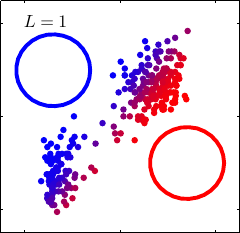
\includegraphics[width=0.40\columnwidth]{resources/em/EM1.png}
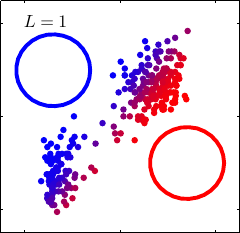
\includegraphics[width=0.21\textwidth]{resources/em/EM1.png}
}\quad
\subfigure[]{
% 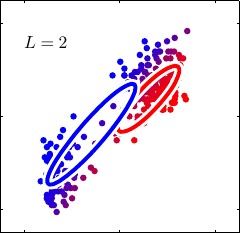
\includegraphics[width=0.40\columnwidth]{resources/em/EM2.png}
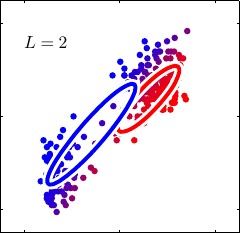
\includegraphics[width=0.21\textwidth]{resources/em/EM2.png}
}\quad
\subfigure[]{
% 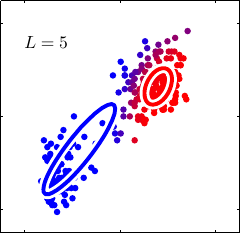
\includegraphics[width=0.40\columnwidth]{resources/em/EM3.png}
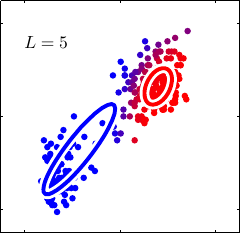
\includegraphics[width=0.21\textwidth]{resources/em/EM3.png}
}\quad
\subfigure[]{
% 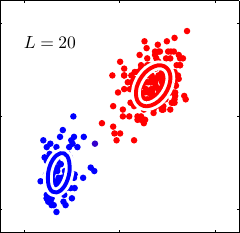
\includegraphics[width=0.40\columnwidth]{resources/em/EM4.png}
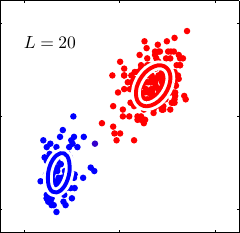
\includegraphics[width=0.21\textwidth]{resources/em/EM4.png}
}\quad
\caption{
Visualization of Expectation-Maximization algorithm \cite{bishopPatternRecognitionMachine2006}.
(a) Clusters are randomly initialized. 
(b) Cluster centers are updated according to the initial assignment (M step).
(c), (d) Expectation and Maximization steps are repeated until convergence.
}
\label{fig:em}
\end{figure}    

\end{secDefinition}

Gaussian Mixture Models suffer from severe overfitting problems in the form of single-point collapse and the fact that the number of clusters needs to be known a priori.
Bayesian parametric (BP) and non-parametric (BNP) mixture models aim to solve these issues by introducing prior distributions governing the model parameters ($\pi, \mu, \boldsymbol{\Sigma}$) and using maximum a priori (MAP) instead of maximum likelihood estimation. 

\begin{secDefinition}[\textbf{Dirichlet Process Mixture Model}] \label{sec:dpmm}
Dirichlet process mixture model (DPMM) is a part of BNP mixture models which finds a clustering solution when $K$ is unknown. 
DPMM extends GMM as it is an infinite mixture model \cref{eq:dpmm} with the Dirichlet process as prior distribution on the number of clusters \cref{eq:prior_dir}. 
Here hyperparameter $\alpha_0$ is the concentration parameter referring to the prior amount of observations associated with each component, and $\Gamma$ refers to the mathematical function "gamma" which in its essence is a generalization of the factorial function that can deal with any real number $>0$.
The cluster parameters $\theta$ are assumed to be i.i.d. and are drawn from a prior distribution. 
In our case, Normal Wishart Distribution (NW) \cref{eq:prior_nw} where hyperparameters $\kappa$ and $\nu$ represent the concentration parameter and degrees of freedom of the Wishart distribution respectively. 
The data is parameterized by the data mean $\mu$ and $\boldsymbol{\Lambda}$ which is the precision matrix (inverse of the covariance matrix $\boldsymbol{\Sigma}$).

\begin{align}
p(\boldsymbol{x}) &=\sum_{i=1}^{\infty} \pi_{i} \mathcal{N}\left(\boldsymbol{x}, \boldsymbol{\mu}_{i}, \boldsymbol{\Lambda}^{-1}\right) \label{eq:dpmm} \\
p(\boldsymbol{\pi}) &= \operatorname{Dir}\left(\boldsymbol{\pi}; \boldsymbol{\alpha}_{0}\right) = \frac{\Gamma(\alpha_0)}{\prod_{i=1}^{K} \Gamma(\alpha_0) } \prod_{i=1}^{K} \pi_{i}^{\alpha_{0}-1} \label{eq:prior_dir} \\
% C\left(\boldsymbol{\alpha}_{0}\right) \prod_{k=1}^{K} \pi_{k}^{\alpha_{0}-1} \label{eq:prior_dir} \\
p(\boldsymbol{\mu}, \boldsymbol{\Lambda}) &= \operatorname{NW}(\boldsymbol{\mu}, \boldsymbol{\Lambda}; \kappa_0, \mu_0, \nu_0, \boldsymbol{W}_0) \notag\\
&= \prod_{i=1}^{K} 
\underbrace{\mathcal{N}\left(\boldsymbol{\mu}_{i} \mid \mu_{0},\left(\kappa_{0} \boldsymbol{\Lambda}_{i}\right)^{-1}\right)}_{p(\mu_i | \boldsymbol{\Lambda}, \kappa_0, \mu_0)}
\underbrace{\mathcal{W}\left(\boldsymbol{\Lambda}_{i} \mid \mathbf{W}_{0}, \nu_{0}\right)}_{p(\boldsymbol{\Lambda}|\mathbf{W}_0, \nu_0)}
\label{eq:prior_nw}
\end{align}

The prior parameters $\alpha_0, \kappa_0$, and $\nu_0$ are set to a predetermined values, whereas prior parameters $\mu_0$ and $W_0$ are calculated on a sample of the full dataset using \cref{eq:nw_mu,eq:nw_W}. Here $\alpha_0, \nu_0,  \kappa_0 \in \mathbb{R}^+$ and $\nu_0 > d + 1$.

\begin{align}
\overline{\mathbf{x}}_{i} &=\frac{1}{N_{i}} \sum_{n=1}^{N} r_{n i} \mathbf{x}_{n} \label{eq:prior_comp_mu} \\
\mathbf{S}_{i} &=\frac{1}{N_{i}} \sum_{n=1}^{N} r_{n i}\left(\mathbf{x}_{n}-\overline{\mathbf{x}}_{i}\right)\left(\mathbf{x}_{n}-\overline{\mathbf{x}}_{i}\right)^{\mathrm{T}} \label{eq:prior_comp_cov}
\end{align}

EM can similarly be used to approximate solutions for DPM models. 
During the E step \cref{eq:prob_assignment} is once again used to estimate the assignments. 
While during the M step \cref{eq:prior_comp_mu,eq:prior_comp_cov} equations analogous to \cref{eq:gm_mu,eq:gm_cov} are used to estimate the data covariance and data mean.
Subsequently the following closed form equations are used to compute posterior parameters for the given prior \cref{eq:nw_kappa,eq:nw_mu,eq:nw_W,eq:nw_nu,eq:dir_pi}.
Given the posterior parameters, the new cluster parameters are inferred using \cref{eq:nw_mu,eq:nw_cov}.
When $\alpha_0$, $\kappa_0$, and $\nu_0$ are much smaller than $N$, the posterior distribution will be influenced primarily by the data rather than the prior.
We use $\lambda$ to denote computed posterior parameters.

\begin{align}
\pi_i &= \frac{N_i}{\sum_{k=1}^k N_i + \alpha_0} \label{eq:dir_pi} \\
\kappa_{i} &=\kappa_{0}+N_{i} \label{eq:nw_kappa} \\
\mu_{i} &=\frac{1}{\kappa_{i}}\left(\kappa_{0} \mu_{0}+N_{i} \overline{\mathbf{x}}_{i}\right) \label{eq:nw_mu} \\
\mathbf{W}_{i}^{-1} &=\mathbf{W}_{0}^{-1}+N_{i} \mathbf{S}_{i}+\frac{\kappa_{0} N_{i}}{\kappa_{0}+N_{i}}\left(\overline{\mathbf{x}}_{i}-\mu_{0}\right)\left(\overline{\mathbf{x}}_{i}-\mu_{0}\right)^{\mathrm{T}} \label{eq:nw_W} \\
\nu_{i} &=\nu_{0}+N_{i} \label{eq:nw_nu} \\
\boldsymbol{\Sigma}_i &= \frac{\nu \mathbf{W}_{i}^{-1}}{\nu - d + 1} \label{eq:nw_cov}
\end{align}

The described implementation solves overfitting and cluster count, though it is an incomplete one since in practice the cluster count has a defined upperbound $K$ (computationally and storage-wise).
While the clusters can get pushed out of existence, no additional clusters can be created.
To solve this issue many variants of DPMM have been proposed utilizing the Chinese Restaurant process, Collapsed Weight sampling, etc. 
We focus on the split/merge sampling algorithm introduced by Chang and Fisher III (DPMMSC) \cite{changParallelSamplingDP2013a}.
For an exhaustive discussion, we refer interested readers to \cite{bishopPatternRecognitionMachine2006, changSamplingComputerVision}.

DPMMSC exploits an alternate perspective in which DPMM is defined as a Monte Carlo Markov Chain if all the chosen priors are conjugate (i.e. prior distribution is in the same form as the posterior distribution).
The stationary distribution is defined by the probability of cluster parameters given the data observations \cref{eq:nw_stationary}.
Intuitively in this approach sampling methods are used to approximate the E step of EM by sampling from the current estimate of posterior distribution $p(\mathbf{z}|\mathbf{X}, \theta^{\text{old}})$ (proposal distribution), where during M step the new state $\theta$ is found.
A similar methodology is employed to transition between different values of $K$ by proposing $\theta$ directly.
As proposal space is unmanageably large, a greedy strategy is employed to propose the most promising states.

\begin{align}
    H_s &= \frac{
    \alpha \Gamma (N_{i_1}) p(X_{i_1}; \lambda_{i_1}) \Gamma (N_{i_2}) p(X_{i_2}; \lambda_{i_2})}{
    \Gamma (N_i) p(X_{i}; \lambda_i)} \label{eq:hastings_sratio}\\
    p(\mu_i, \boldsymbol{\Sigma}_i | \mathbf{X}_i) &= \operatorname{NW}(\boldsymbol{\mu}, \boldsymbol{\Lambda}; \kappa_0, \mu_0, \nu_0, \boldsymbol{W}_0) \label{eq:nw_stationary} \\
    p(\mathbf{X}; \lambda) &= \int p\left(\mathbf{X} \mid \boldsymbol{\mu}_{i}, \boldsymbol{\Sigma}_{i}\right) p\left(\boldsymbol{\mu}_{i}, \boldsymbol{\Sigma}_{i} ; \lambda\right) d\left(\boldsymbol{\mu}_{i}, \boldsymbol{\Sigma}_{i}\right) \notag \\
    &=\frac{1}{\pi^{\frac{N d}{2}}} 
    \frac{\Gamma_{d}\left(\nu_0 / 2\right)}{\Gamma_{d}(\nu_i / 2)} 
    \frac{|\nu_0 \boldsymbol{\Lambda}_0|^{\nu_0 / 2}}{\left|\nu_i \boldsymbol{\Lambda}_{i}\right|^{\nu_i / 2}}\left(\frac{\kappa_i}{\kappa_0}\right)^{d / 2} \label{eq:data_prob}
\end{align}

For each supercluster $i$, two auxiliary subclusters are defined with parameters $\theta_{i_1}$ and $\theta_{i_2}$ forming a two-component GMM.
Once subclusters are in a converged state, the split proposals are made given the supercluster and its two subcomponents.
Similarly, supercluster merges are proposed by picking $k$ nearest candidates for each supercluster.

The proposed candidates are either accepted or rejected by the Metropolis-Hastings (MH) algorithm moving the model to the next state.
As the split acceptance ratio $H_s$ is defined by the probability of data being sampled from the split state in contrast to the current state \cref{eq:hastings_sratio}.
Analogously, the merge ratio is its inverse, namely $\frac{1}{H_s}$.
\cref{eq:gmm_ll,eq:dir_pi,eq:prior_nw,eq:nw_stationary} are used to derive the marginal probability of data being generated by parameter set $\lambda$ given prior parameters \cref{eq:data_prob} (note that $\pi$ refers to the mathematical constant, and $\Gamma_d$ refers to mathematical function digamma).
%
The proposals are considered once the supercluster model has converged. If no proposal is accepted, then DPMMSC is considered as converged.
\end{secDefinition}

\begin{secDefinition}[\textbf{Graph Convolutional Neural Networks}]
Graph Convolutional Neural Networks (GCN) \cite{kipfSemiSupervisedClassificationGraph2017, hamiltonInductiveRepresentationLearning2017, kazemiRepresentationLearningDynamic2020} generate node embeddings given a spatial filter which is applied as a convolution given each node's graph neighborhood.
The convolution operation enables GCNs to propagate structural information of graphs throughout the network (referred to as message-passing). 
By layering this process, the receptive field of each node expands to its k-hop neighborhood.

Suppose $H_t^l$ is the representation of node $t$ at layer $l$, a forward step of the message-passing procedure is defined as \cref{eq:gnn_forward} where $N(t)$ is $t$'s neighboring node set and $\mathcal{E}(s, t)$ is the set of edges between nodes $t$ and its neighbor $s$. Here the operator $\operatorname{\textbf{Message}}(\cdot)$ extracts useful information from the neighboring source nodes $s$, while the $\operatorname{\textbf{Aggregate}}(\cdot)$ operator gathers the neighborhood information via some aggregation operator such as \textit{mean}, \textit{sum} or \textit{max} to get contextualized representation of $t$.

\begin{align}
    H_t^{(l)} = \underset{\forall s \in N(t), \forall e \in \mathcal{E}(s, t)}{\operatorname{\textbf{Aggregate}}} \left[\operatorname{\textbf{Message}}\left( H_s^{(l-1)}, e, H_t^{(l-1)} \right) \right] \label{eq:gnn_forward}
\end{align}

The time complexity to run a forward step over the entire training set is $O(|\mathcal{V}| \cdot deg \cdot d^2)$ where $deg$ refers to the average node degree.
While $deg \ll |\mathcal{V}|$ is true for most graphs, a vital optimization step is to sample a fixed size $N_v$ ensuring that $deg$ is bounded by a constant.
\end{secDefinition}

\begin{secDefinition}[\textbf{Heterogeneous Graph Transformer}]
\begin{figure}[!ht]
\centering
% 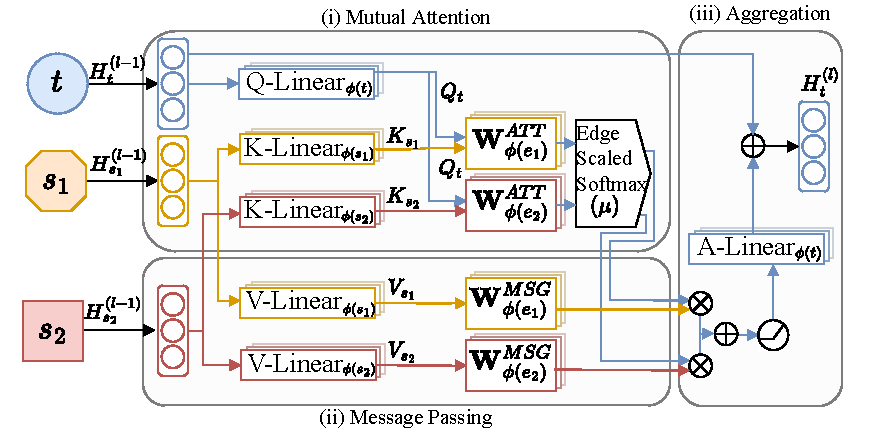
\includegraphics[width=\columnwidth]{resources/hgt.png}
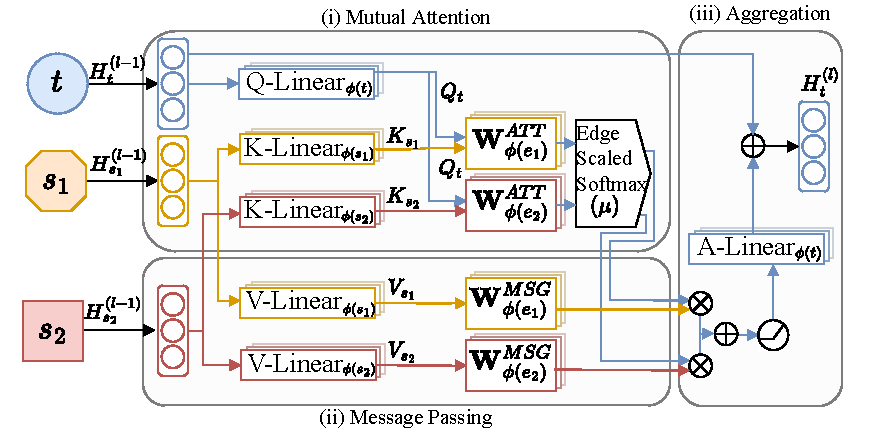
\includegraphics[width=0.8\columnwidth]{resources/hgt.pdf}
\caption{
    Visualization of a Heterogeneous Graph Transformer Layer. Given target node $t$ and neighboring source nodes $s_1$ and $s_2$ by edges $e_1$ and $e_2$, mutual attention and messages are computed. Within aggregation step the messages are attended and combined with previous target node embedding $H^{(l-1)}_t$ resulting in the new embedding vector $H^{(l)}_t$
}
\label{fig:hgt}
\end{figure}    

Classical GCNs focus mainly on homogeneous graphs. 
A fair amount of works describe ways to adapt existing algorithms by introducing a $\operatorname{\textbf{Message}}$ step parameterized by meta-topological types.
Based on the observation that the value of different connections varies given a node type, attention-based mechanisms are introduced into the aggregation process.
Inspired by success in NLP Heterogeneous Graph Transformer (HGT) \cite{huHeterogeneousGraphTransformer2020} adopts the transformer architecture \cite{vaswaniAttentionAllYou2017} by calculating mutual attention based on representation and meta-types of source, target and relation information.

\begin{align}
    H_t^l = \underset{\forall s \in N(t), \forall e \in \mathcal{E}(s, t)}{\operatorname{\textbf{Aggregate}}} \left[
    \operatorname{\textbf{Attention}}\left( s, e, t \right) \cdot
    \operatorname{\textbf{Message}}\left( s, e, t \right) 
    \right] \label{eq:hgt_forward}
\end{align}

HGT consists mainly of three components, (i) mutual attention possession performance of each source node, (ii) message passing extracts information from source nodes, and (iii) target-specific aggregation which combines the neighborhood messages.
A general form for a forward pass is defined as \cref{eq:hgt_forward} and is visualized in \cref{fig:hgt}.

The attention vector is calculated by mapping source node $s$ into Key $K$ and target node $t$ into a Query $Q$ vectors \cref{eq:hgt_K,eq:hgt_Q}.
A single head attention vector is calculated as inner product similarity vector between Key $K$ and Query $Q$ vectors (See \cref{eq:hgt_att_head}) given a relation specific interaction matrix, where prior tensor $\mu \in \mathbb{R}^{|\mathcal{A}| \times |\mathcal{R}| \times |\mathcal{A}|}$ denotes significance of each relation triplet. 
$K(s)$ and $Q(t)$ are computed as projections of source $s$ and target $t$ nodes respectively \cref{eq:hgt_K,eq:hgt_Q}.
The final attention vector results from a concatenation of $h$ attention heads per source node \cref{eq:hgt_att}.

\begin{align}
    \operatorname{\textbf{Attention}}_{H G T}(s, e, t) &= \underset{\forall s \in N(t)}{\operatorname{Softmax}} \left(\underset{i \in[1, h]}{\|} \operatorname{\textit{ATT-Head}}^{i}(s, e, t)\right) \label{eq:hgt_att} \\
        \operatorname{\mathit{ATT-Head}}^{i}(s, e, t) &=\left(K^{i}(s) W_{\psi(e)}^{A T T} Q^{i}(t)^{T}\right) \cdot \frac{\mu_{\langle\phi(s), \psi(e), \phi(t)\rangle}}{\sqrt{d}}  \label{eq:hgt_att_head} \\
        K^{i}(s) &=\operatorname{K-Linear}_{\phi(s)}^{i}\left(H^{(l-1)}_s\right) \label{eq:hgt_K} \\
        Q^{i}(t) &=\operatorname{Q-Linear}_{\phi(t)}^{i}\left(H^{(l-1)}_t\right) \label{eq:hgt_Q}
\end{align}

Similarly, the multi-head message is computed by applying type-dependent projection ($\operatorname{V-Linear}$) to the input source node representation and transforming it using the edge type matrix $W_{\psi(e)}^{MSG} \in \mathbb{R}^{\frac{d}{h} \times \frac{d}{h}}$ to incorporate the relation dependency into the result \cref{eq:hgt_msg_head}. 
In both operations, edge interaction matrices and the head-specific type projection matrices are shared to minimize the number of used parameters.  

\begin{align}
    \operatorname{\textbf{Message}}_{HGT}(s, e, t) &=\underset{i \in[1 \ldots h]}{\|} \operatorname{\textit{MSG-Head}}^{i}(s, e, t) \label{eq:hgt_msg} \\
        \operatorname{\mathit{MSG-Head}}^{i}(s, e, t) &=\operatorname{V-Linear}{ }_{\phi(s)}^{i}\left(H^{(l-1)}_s\right) W_{\psi(e)}^{MSG} \label{eq:hgt_msg_head}
\end{align}

Finally, during the aggregation step, the calculated attention is applied to neighborhood messages and summed into the neighborhood representation vector \cref{eq:hgt_neigh}.
The final node representation vector $H^{(l)}_t$ results from the summation of the projected neighborhood vector into the target node space and the previous representation of the target vector \cref{eq:hgt_agg}.

\begin{align}
    \widetilde{H}^{(l)}_t &=\underset{\forall s \in N(t)}{\oplus}\left(\operatorname { \textbf{Attention} }_{HGT}(s, e, t) \cdot \operatorname{\textbf{Message}}_{HGT}(s, e, t)\right) \label{eq:hgt_neigh} \\
    H^{(l)}_t &=\operatorname{A-Linear}_{\phi(t)}\left[\sigma\left(\widetilde{H}^{(l)}_t\right)\right]+H^{(l-1)}_t \label{eq:hgt_agg}
\end{align}

See \cref{fig:hgt} for a visualization of a forward pass of single layer HGT. 

\end{secDefinition}

\vspace{3mm}
\noindent\textbf{Problem formulation.} 
Given a multimodal graph $G$, our goal is to learn a node embedding function $\zeta: G_{v} \rightarrow \mathbb{R}^{d}$ which given a $k$-hop neighborhood subgraph $G_{v}$ of node $v$ produces a $d$-dimensional embedding vector $Z_v$.
%The embedding $Z_v$ should minimize the proximity to other nodes embeddings given they are topological and/or temporal context neighbors of node $v$.
The objective is to minimize the distance between embedding $Z_v$ to other node embeddings, given that they are topological and/or temporal context neighbors of node $v$.
Taking into account incompleteness constraints (\cref{def:incompleteness_constraints}), $\zeta$ should work under any valuation of $(\mathbf{1}_{\mathcal{X}(v)}, \mathbf{1}_{\mathcal{T}(v)}, \mathbf{1}_{\mathcal{V}(v)})$.
We also aim to find community parameters $\mathbf{\theta} = \{\mathcal{N}(\mu_1, \Sigma_1), ..., \mathcal{N}(\mu_K, \Sigma_K)\}$ and node-to-community assignment $\mathbf{z} \in \{0, .., K\}^{|\mathcal{V}|}$ such that their members have a low inter-proximity in contrast to other nodes.
Finally, the found community count $K$ should approximate the ground truth number of communities.
\chapter{The Proposed Approach}\label{sec:approach}

\begin{figure*}[ht!]
\centering
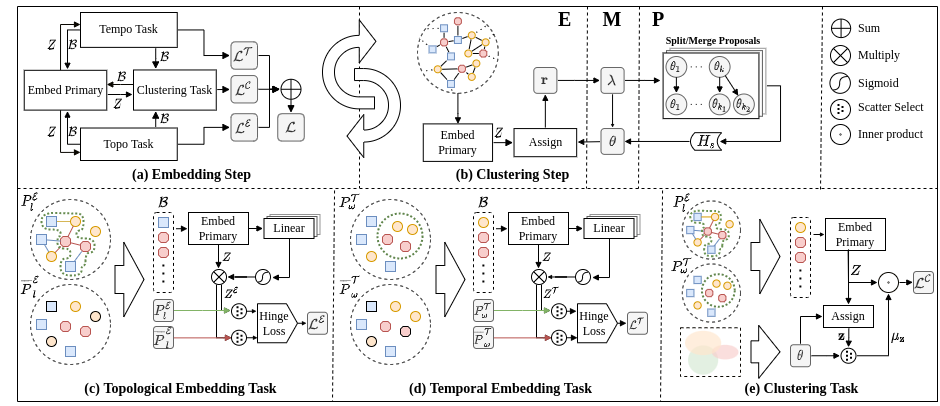
\includegraphics[width=\textwidth]{resources/framework.png}
\caption{Overview of the MGTCOM framework.
(a) In the embedding step primary embeddings are used in auxiliary tasks to construct the multi-objective loss. 
(b) Clustering step updates clustering by alternating between Expectation (\textbf{E}), Maximization (\textbf{M}), and Proposal (\textbf{P}) steps.
(c) In the topological (topo) embedding task, random walk sampling and feature-wise attention minimize inter-node proximity.
(d) In the temporal (tempo) embedding task, ballroom walk sampling and feature-wise attention minimize proximity between temporally related nodes.
(e) Clustering task adds community awareness to the embeddings by minimizing proximity between nodes within the same cluster.
}
\label{fig:framework}
\end{figure*}

We present our framework for Community Detection in Temporal Multimodal Graphs (MGTCOM) that learns multimodal representation vectors for graph nodes and detects communities in tandem.
We achieve this by leveraging heterogeneous graph transformers \cite{huHeterogeneousGraphTransformer2020} to learn a primary node embedding function $\zeta$. In order to handle the incompleteness constraints, we introduce an auxiliary embedding vector $E$ for known (or seen) nodes with missing features.
Next, we learn task-specific node representation for topological and temporal information by combining primary embeddings with task-specific transformation/attention and context sampling. 
As we utilize random walks for topological context sampling, we introduce its analogue as an unbiased temporal window sampling algorithm for temporal context collection.
Finally, we adopt DPMM for community detection and close the loop by introducing cluster-based loss to ensure the graph embeddings are \textit{community-aware}.
%
MGTCOM consists of three major components (as can be seen in \cref{fig:framework}): primary embedding module, (a) task-specific learning, and (b) community detection/clustering module. MGTCOM also has a graph sampling component.  In the following, we describe the components in detail. 

\section{Primary embedding module}
The central component of our framework is responsible for inferring the primary representation vector $Z_v$ given a node $v \in \mathcal{V}$ in a graph $G$. 
%
Motivated by the success of inductive GCN-based methods \cite{hamiltonInductiveRepresentationLearning2017, yingGraphConvolutionalNeural2018, huHeterogeneousGraphTransformer2020}, we build our architecture by combining $L$ graph convolution layers ($\mathit{HeteroConv}$ or HGCN) and a graph subsampler ($\mathit{HeteroSample}$). 

Specifically, we use the budget-based subgraph sampling algorithm and the heterogeneous graph transformer (HGT) proposed by Hu et al. \cite{huangInformationFusionOriented2022}.
HGT captures topological, meta-topological, and content-based aspects by combining off-the-shelf graph convolution with node type-specific projection and edge type-based attention.

\cref{alg:prim_feat} provides a full overview of the primary embedding algorithm. 
The basic idea is to infer node representation from its k-hop heterogeneous neighborhood subgraph $G_v$ while handling edge cases introduced by the incompleteness constraints (\cref{def:incompleteness_constraints}) in order to handle web-scale multimodal graphs.
The inference starts by sampling a subgraph $G_{\mathcal{B}}$ given a batch of central nodes using the \textit{budget sampling} algorithm on \cref{alg:pe:sampling}.
The \textit{budget sampling} algorithm works by restricting sampled subgraph at each layer given a per node type limit.
For our use case, we define this limit as multiple $|\mathcal{B}|$ to avoid re-tuning its value for each dataset. 
% We use node type bound budget required by \textit{budget sampling} algorithm as a multiple of $|\mathcal{B}|$ for each of the layers to hyperparameter retuning for different datasets.

Once the graph is sampled we split the task of initial feature inference into three cases to handle the incompleteness constraints.
(i) If a feature vector is present, then it is simply projected into the representation space.
(ii) If the node is in the training set while no feature vector is present, then its representation is drawn from the \textit{auxiliary embedding} matrix $\mathbf{E}$. To avoid overreliance on the embeddings in preference for feature vectors we apply dropout on the resulting representation.
(iii) Finally, if an unseen node without a feature vector is encountered, the zero vector (denoted as $0_d$) is used, indicating that its feature vector has zero weight during the aggregation step of the graph convolution.
Note that for large datasets, it may not be feasible to keep a full auxiliary embedding matrix in memory. 
In \cref{sec:abl:aux_emb} we explore a setting where auxiliary embeddings are limited to a subset of important nodes.

\begin{algorithm}[!t]
    \small
    \caption{Batchwise primary node embedding}\label{alg:prim_feat}
    \SetKwFunction{procPrimary}{EmbedPrimary}

    \SetKwProg{myproc}{Procedure}{}{}
    \myproc{\procPrimary{}}{
        \KwIn {
            multimodal graph $G = (\mathcal{V}, \mathcal{E}, \mathcal{A}, \mathcal{R}, \mathcal{X})$,
            mini-batch $\mathcal{B} \subseteq \mathcal{V}$,
            auxiliary node embedding $\mathbf{E} \in \mathbb{R}^{N_{\bar{\mathcal{X}}} \times d }$
            where $N_{\bar{\mathcal{X}}} = |\{v|v \in \mathcal{V}, \mathbf{1}_{\mathcal{X}}(v) = 0\}|$,
            number of convolutional layers $L$
        }
        \KwOut {
            The primary embedding $Z_{\mathcal{B}}$ for nodes in batch $\mathcal{B}$
        }
            $G_{\mathcal{B}}(\mathcal{V}_{\mathcal{B}}, \mathcal{E}_{\mathcal{B}}, \mathcal{A}_{\mathcal{B}}, \mathcal{R}_{\mathcal{B}}, \mathcal{X}_{\mathcal{B}}) \leftarrow \operatorname{HeteroSample}(G, \mathcal{B}, L)$\; \label{alg:pe:sampling}
            \For {$s \in \mathcal{V}_{\mathcal{B}}$} {
                $H_s^{(0)} = \begin{cases}
                    \operatorname{Linear}(\mathbf{x_s}) & \mathbf{1}_{\mathcal{X}}(s) = 1 \\
                    \operatorname{Dropout}(\mathbf{E}_s)& \mathbf{1}_{\mathcal{V}}(s) = 1 \\
                    0_d                                 & \text{otherwise}
                \end{cases}$\; \label{alg:pe:feature_inf}
            }
            \For {$l = 1$ \KwTo $L$} {
                $H^{(l)} = \operatorname{GeLU}(\operatorname{HeteroConv}(G_{\mathcal{B}}, H^{(l-1)}))$\; \label{alg:pe:conv}
            }
            $Z_{\mathcal{B}} = \{H^{(L)}_t | t \in \mathcal{B} \}$\; \label{alg:pe:batch}
        \Return {$Z_{\mathcal{B}}$}
    }
\end{algorithm}


On \cref{alg:pe:conv}, given the subgraph $G_\mathcal{B}$ and the initial representation vector $H^{(0)}$,  $L$ layers of HGT graph convolutions are applied.
Each layer uses the representation vector of the previous layer and feeds its output through a $\operatorname{GeLU}$ \cite{hendrycksGaussianErrorLinear2020} activation function (See \cref{sec:abl:hyperparam} for performance comparison).
Finally, the output vectors at the $L^\mathit{th}$ layer are used as primary representation vectors and output for each query node in the batch on \cref{alg:pe:batch}. 

\section{Multi-task representation learning}
During task-specific learning we focus on two main tasks capturing the intricacies of multimodal networks.
The topological task identified by $\mathcal{E}$ focuses on minimizing the representation distance between nodes that are proximate within the network.
Analogously, the temporal task $\mathcal{T}$ focuses on minimizing the distance between nodes that co-occur at the same timeframes.
While fundamentally different since the tasks are trained in parallel, they benefit from weight sharing and from node sharing during primary embedding as the subgraph batches are centered around the same nodes.

\subsection{Task-based attention}
An important observation is that while temporal and topological communities are both important during analysis, they are not always correlated.
In fact, in most of the benchmarking datasets such as Cora and DBLP temporal features and graph structure show low correlation.
While it is very rare that contentual features are completely independent of topology and temporality, we describe a general implementation that can be applied to such a case. 

Given the above observation, we admit that it may not be possible to train a model that excels at both tasks.
To work around this issue while still capturing both tasks in a single embedding vector we introduce \textit{task-based attention}.
The basic idea is that while primary embedding extracts suitable features from the multimodal network, task-specific attention selects the most relevant of these features for the task at hand.
%
Inspired by transformers \cite{vaswaniAttentionAllYou2017} we define multi-head attention to capture various feature patterns \cref{eq:task_attention}.
The task-based transformation function is defined as \cref{eq:task_transform} where the primary representation vector is attended to using a simple matrix multiplication operation.
We specialize this function for topological task as $f^{\mathcal{E}}(\mathbf{Z})$ producing $\mathbf{Z}^{\mathcal{E}}$ and temporal task $f^{\mathcal{T}}(\mathbf{Z})$ producing $\mathbf{Z}^{\mathcal{T}}$.

\begin{align}
    f^{task}(\mathbf{Z}) &= \mathbf{Z} \cdot \operatorname{\textit{ATT}}^{task}(\mathbf{Z}) \label{eq:task_transform}  \\
    \operatorname{\textit{ATT}}^{task}(\mathbf{Z}) &= \underset{i \in [1..h]}{\|} \sigma \left[ \operatorname{Linear}^i_{task}(\mathbf{Z}) \right] \label{eq:task_attention}
\end{align}

\subsection{Objective function} \label{sec:obj_fn}
In order to learn model parameters in an unsupervised way, we define contrastive loss.
Task-specific positive context sample $P$ and a negative context sample $\bar{P}$, both sharing a central query node $q$ are used to construct positive $(q, p)$ and negative $(q, n)$ node pairs respectively.
We define a max-margin-based loss function (\cref{eq:max_margin}) which aims to maximize the inner product similarity between the query and positive examples.
On the other hand, the inner product of query and negative samples is minimized to be smaller than that of the positive samples by some predefined value of $\Delta$ (see \cref{sec:abl:hyperparam} hyperparameter experiments).
In our tests, we found that averaging similarity over positive samples within the max loop helps to smoothen out the noise caused by context sampling \cref{eq:mm_mean_aff}.

\begin{align}
    \operatorname{MM-Loss}(\mathbf{Z}, P, \bar{P}, q) &= \max_{n \in \bar{P}} \left\{0, \mathbf{Z}_q \mathbf{Z}_n - \widetilde{\mathbf{Z}_q \mathbf{Z}_p} + \Delta \right\} \label{eq:max_margin} \\
    \widetilde{\mathbf{Z}_q \mathbf{Z}_p} &= \frac{1}{|P|} \sum_{p \in P } \left(\mathbf{Z}_q \mathbf{Z}_p \right) \label{eq:mm_mean_aff}
\end{align}

% ====================================
\subsection{Temporal context sampling}\label{sec:tempo_sampling}
\begin{figure*}[htbp]
\centering
\subfigure[]{
% 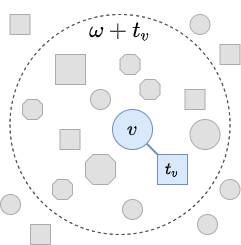
\includegraphics[width=0.42\columnwidth]{resources/ballroom/br2.png}
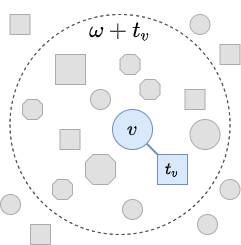
\includegraphics[width=0.21\columnwidth]{resources/ballroom/br2.png}
}\quad
\subfigure[]{
% 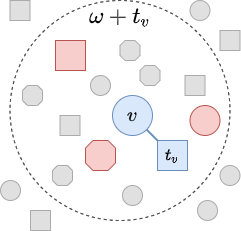
\includegraphics[width=0.42\columnwidth]{resources/ballroom/br3.png}
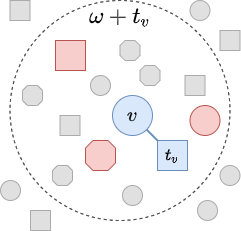
\includegraphics[width=0.21\columnwidth]{resources/ballroom/br3.png}
}\quad
\subfigure[]{
% 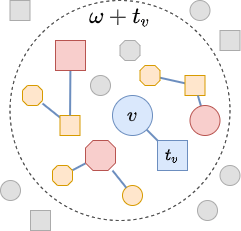
\includegraphics[width=0.42\columnwidth]{resources/ballroom/br4.png}
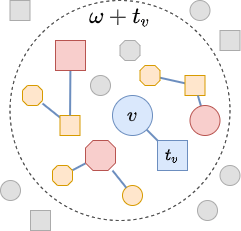
\includegraphics[width=0.21\columnwidth]{resources/ballroom/br4.png}
}\quad
\subfigure[]{
% 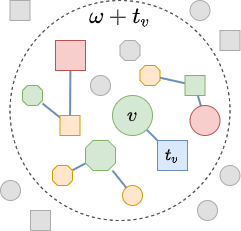
\includegraphics[width=0.42\columnwidth]{resources/ballroom/br5.png}
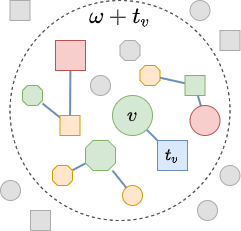
\includegraphics[width=0.21\columnwidth]{resources/ballroom/br5.png}
}\quad

\caption{
    Visual overview of Ballroom Walk temporal sampling algorithm.
    (a) The sampling timestamp $t_v$ for query node $v$ is inferred given the nearest neighbor if the node is static (blue). The relative time window is determined as $\omega + t_v$.
    (b) The root context nodes are sampled from the relative time window (red).
    (c) Context is extended with temporal random walks from the root nodes (yellow).
    (d) The context path is sampled from the collected context (green).
}
\label{fig:br}
\end{figure*}

Temporal features are often not correlated with network topology.
We propose a separate context sampling function that, given a query node and an interval window $\omega$, returns other nodes occurring within the same time window. 
The interval window $\omega$ is determined by using the dataset statistics as a fraction of the complete time range $\mathcal{T}$.
By picking a small enough interval window, a fine-grained continuous-time representation vector can be learned.
This is because additional granularity is achieved by centering the sample around the query node.
% as during sampling it is shifted to be centered around the query node.

Edge cases arising from the incompleteness constraints need to be handled where the nodes are missing timestamps $\mathbf{1}_{\mathcal{T}} = 1$.
While the usual semantic approach is to consider these nodes omnipresent (static), the naive window sampling methods quickly get congested with static to static context pairs.
Our aim is to alleviate this issue using biased sampling in favor of non-static pairs.

We start by introducing the temporal random walk procedure shown in \cref{alg:tempo_rw} which enforces standard random walks over the network to stay within a predetermined temporal window $\omega^*$.
Here random walk of size $l$ is constructed by picking a randomly connected node to the current head node (\cref{alg:trw:neighbors}) within a time window.
If no such node is present, then the random walk is restarted from any already picked node \cref{alg:trw:restart}.
The walk is extended with a new head node until it reaches the desired length.

\begin{algorithm}[!t]
    \small
    \caption{Temporal Random Walk}\label{alg:tempo_rw}
    \SetKwFunction{algo}{BallroomWalk}
    \SetKwFunction{proc}{TemporalRW}
    \SetKw{KwGoTo}{go to}
    
    \setcounter{AlgoLine}{0}
    \SetKwProg{myproc}{Procedure}{}{}
    \myproc{\proc{}}{
    \KwIn {
        center node $v$,
        temporal window $\omega^*$
    }
    \KwOut {
        Temporal random walk $P_l$
    }
        Initialize $P_l$ = $[]$\; 
        $(u, t_u) = (v, \varnothing)$\;
        \For {$i = 1$ \KwTo $l$} {
            $N(u) = \{w| 
                w \in \mathcal{V}, 
                (u, w) \in \mathcal{E},
                \tau(w) \cap \omega^* \neq \emptyset
            \}$\;\label{alg:trw:neighbors}
        
            \If (\tcc*[h]{Restart on dead end}){$N(u) = \emptyset$}{
                $(u, t_u) = (v, t_v)$\; \label{alg:trw:restart}
                \KwGoTo \ref{alg:trw:neighbors}\;
            }

            $w \sim N(u)$\; \label{alg:trw:sample}
            $t_u = \max \left\{ t_u, \min{ \tau(w)} \right\}$\;
            $u = w$\;

            $P_{l}.append((u, u_t))$\;
        }

        \KwRet $P_l$
    }
\end{algorithm}

Utilizing the idea of temporal random walks we propose our own sampling method "Ballroom Walk" whose outline is shown in \cref{alg:ballroom_walk}.
% An outline of our proposed sampling method "Ballroom Walk" is shown in \cref{alg:ballroom_walk}.
It starts by inferring the sampling timestamp $t_v$ by picking a random timestamp the query node $v$ occurs in.
If the node is static, the timestamp of its nearest neighbor reachable through temporal random walk is selected (\cref{alg:brw:infer_t}).
To reliably sample the temporal neighborhood, $n$ root nodes ($w$) are picked occurring in the time-window relative to the sampling timestamp on \cref{alg:brw:neighborhood}.
Temporal context $C$ is constructed by collecting temporal random walks starting from root nodes $w$ given a relative time window $\omega + t_v$ on \cref{alg:brw:context}.
Finally, $l$ long context paths are created as random subsets of $C$.
Note that because a sampled context is valid for all member nodes, random walk-like throughput optimization can be used by setting a larger window length than context size~\cite{perozziDeepWalkOnlineLearning2014}.

\begin{algorithm}[!t]
    \small
    \caption{Ballroom walk sampling}\label{alg:ballroom_walk}
    \SetKwFunction{algo}{BallroomWalk}
    \SetKwFunction{proc}{TemporalRW}
    \SetKw{KwGoTo}{go to}
    
    \SetKwProg{myalg}{Algorithm}{}{}
    \myalg{\algo{}}{
    \KwIn {
        %temporal graph $G = (\mathcal{V}, \mathcal{E}, \mathcal{T})$,
        multimodal graph $G = (\mathcal{V}, \mathcal{E}, \mathcal{A}, \mathcal{R}, \mathcal{X})$,
        relative temporal window $\omega$,
        walks per node $n$,
        walk length $l$,
        center node $v$, 
    }
    \KwOut {
        Temporal $n$ random walks $P_l$
    }
        Initialize $C$\;
        $t_v = \begin{cases}
            t_v \sim \tau(v)                                            & \mathbf{1}_{\mathcal{T}}(v) = 1 \\
            % [(\_, t_v), ...] \leftarrow \proc{$v$, $(-\infty, \infty)$}     & \text{otherwise}
            \proc{$v$, $(-\infty, \infty)$}.first()     & \text{otherwise}
        \end{cases}$\; \label{alg:brw:infer_t}
        $N(v) = \{w|
            w \in \mathcal{V}, 
            \tau(w) \cap \omega + t_v \neq \emptyset
        \}$\; \label{alg:brw:neighborhood}
        \For {$i = 1$ \KwTo $n$}{
            $w \sim \mathcal{N}$\;
            $C = C \cup \proc{$w$, $\omega + v_t$}$\; \label{alg:brw:context}
        }
        \texttt{RandomPermute}($C$)\;

        \For {$i = 1$ \KwTo $n$}{
            $P_l = \{C_j | i \cdot l \leq j < i \cdot l+l\}$\; \label{alg:brw:walks}
            \KwRet $P_l$\;
        }
    }{}
    
    % \setcounter{AlgoLine}{0}
    % \SetKwProg{myproc}{Procedure}{}{}
    % \myproc{\proc{}}{
    % \KwIn {
    %     center node $v$,
    %     temporal window $\omega$
    % }
    % \KwOut {
    %     Temporal random walk $P_l$
    % }
    %     Initialize $P_l$\; 
    %     $(u, t_u) = (v, \varnothing)$\;
    %     \For {$i = 1$ \KwTo $l$} {
    %         $\mathcal{N} = \{w| 
    %             w \in \mathcal{V}, 
    %             (u, w) \in \mathcal{E},
    %             (\tau(u) \cap \tau(w) \cap \omega ) \neq \emptyset
    %         \}$\;\label{all:tempo_neighbors}
        
    %         \If (\tcc*[h]{Restart on dead end}){$\mathcal{N} = \emptyset$}{
    %             $(u, t_u) = (v, t_v)$\;
    %             \KwGoTo \ref{all:tempo_neighbors}\;
    %         }

    %         $w \sim \mathcal{N}$\;
    %         $t_u = \max \left\{ t_u, \min \tau(w), \tau((u, w)) \right\}$\;
    %         $u = w$\;

    %         $P_{l}.push((u, u_t))$\;
    %     }

    %     \KwRet $P_l$
    % }
\end{algorithm}

Due to timestamp inference, the first- and second-order proximity static to static pairs are ignored.
By only passively sampling omnipresent nodes we mitigate the over-saturation issue while still being fair.
Most importantly the neighborhood of central nodes is being sampled independently of their topology.
By sampling within a temporal window, we avoid not relying on the correlation of temporality with topology.

% ====================================
\subsection{Graph sampling}
The objective of task-specific learning is mainly defined by the context sampling method.
As our method allows for inference of primary and task-specific representations for unseen nodes, we assume that topological, meta-topological and contentual features contain enough information / are correlated with the objective of the tasks.
%
% Topo sampling
To gather the topological context $P^{\mathcal{E}}$, Node2Vec biased random-walk algorithm is utilized \cite{groverNode2vecScalableFeature2016}.
By choosing a low value for its control parameter $q$ we discourage structural/topological equivalence representation in favor of larger neighborhood exploration (depth-first strategy) which is useful for community representation.
% Tempo sampling
Similarly, we use ballroom sampling to collect temporal context $P^{\mathcal{T}}$ of size $l$ as introduced in the previous section.
The negative nodes are collected by sampling random nodes from the graph.
% Sharing
In our framework, the query nodes and negative contexts are shared across both tasks. 
% Similarly, as the tasks are trained in parallel, their loss is combined to facilitate multi-objective optimization (See \cref{alg:pipeline}).

\section{Community detection}
For community detection, we adopt the DPMM split/merge algorithm proposed by Chang and Fisher III \cite{changParallelSamplingDP2013a} as discussed in \cref{sec:dpmm}.
In our implementation, we use Normal Wishart (NW) as a conjugate prior and use variational lower bound in our convergence criteria.
%
Specifically, we monitor the log sum of the variational lower bound \cref{eq:var_lb} for the supercluster and subcluster models. 
The variational lower bound is computed as the product of variational distribution $q(\mathbf{z})$, the normalizing constant of the Dirichlet distribution $B(\alpha_0)$, and the normalizing constant of the Normal Wishart distribution $C(W, \nu)$.
Once its monitored value starts oscillating, then the model has converged and is moved into the proposal state.
If the model parameters remain unchanged during the proposal stage (no split or merge is accepted), then the clustering is complete.

\begin{align}
    \operatorname{Lower-Bound}(r) = 
    \underbrace{\left[ \prod_{n=1}^{N} \prod_{k=1}^K r_{nk} e^{r_{nk}} \right]}_{q(\mathbf{z})}
    \underbrace{\frac{\prod_{i=1}^K \Gamma(\alpha_0)}{\Gamma \left( \sum_{k=1}^K \alpha_0 \right)}}_{B(\alpha_0)}
    \underbrace{2^{\frac{\nu d}{2}} |W|^{\frac{\nu}{2}} \Gamma_d \left(\frac{\nu}{2} \right)}_{C(W, \nu)} \label{eq:var_lb}
\end{align}

The only parameters relevant for our clustering method are the prior hyperparameters (See \cref{sec:dpmm}).
Most of the parameters (i.e. $\alpha$, $\kappa$, and $\nu$) are not very relevant if they are much smaller than the sample count.
We use the $\Sigma_{scale}$ parameter to scale the dataset covariance for more effective control over the strength of the data-bound prior parameters $\mu_0, \Sigma_0$.
In \cref{sec:abl:hyperparam} we provide a more detailed analysis of result sensitivity to prior parameters.

To fit the clustering model we use primary embedding to calculate assignment and posterior parameters as it contains features relevant for both temporal and topological tasks.
While not explored in this thesis, it is worth noting that it is not necessary to have all the embeddings in memory as exact posterior parameters depend on data $\mu$ and $\Sigma$ which can be calculated over multiple batches.

\section{End-to-end approach}
Given a graph embedding, it is straightforward to find communities by performing the embedding and clustering tasks sequentially. 
This approach lacks a unified objective, thus, the node embeddings may not be optimized for community detection.
We extend the objective with cluster-based loss calculated as the distance between node embedding and its assigned cluster $z_v$ \cref{eq:loss_clus}.
This introduces a feedback loop that encourages the model to reinforce community structures while optimizing the topological and temporal objectives \cref{eq:combined_loss}.
%
The influence of three objectives can be controlled using hyperparameters $\beta^{\mathcal{E}}$, $\beta^{\mathcal{T}}$, and $\beta^{\mathcal{C}}$.

\begin{align}
    \mathcal{L}^{C} &= \left\|Z_v - \mu_{z_v} \right\|^2_{\ell 2} \label{eq:loss_clus} \\
    \mathcal{L}^{\mathcal{E}} &= \operatorname{MM-Loss}(\mathbf{Z}, P^{\mathcal{E}}, \bar{P}, v) \label{eq:loss_topo} \\
    \mathcal{L}^{\mathcal{T}} &= \operatorname{MM-Loss}(\mathbf{Z}, P^{\mathcal{T}}, \bar{P}, v) \label{eq:loss_tempo}\\
    \mathcal{L} &= \beta^{\mathcal{E}} \mathcal{L}^{\mathcal{E}} + \beta^{\mathcal{T}} \mathcal{L}^{\mathcal{T}} + \beta^{\mathcal{C}} \mathcal{L}^{\mathcal{C}} \label{eq:combined_loss}
\end{align}


With this closed feedback loop, the training procedure consists of two alternating stages (See \cref{fig:framework} and \cref{alg:pipeline}).
The \textit{embedding optimization} stage (\cref{alg:pipeline:feat_optimization}), is responsible for optimizing the graph embedding function parameters while keeping cluster parameters $\theta$ fixed.
Once the graph embeddings are updated we run $I_c$ clustering/EM steps to optimize cluster parameters $\theta$ while keeping node representations fixed \cref{alg:pipeline:cluster_optimization}. Note that the \textit{representation optimization} stage is run until convergence as part of pretraining beforehand to ensure the clusters are initialized properly.

\begin{algorithm}[t!]
    \small
    \caption{MGTCOM learning pipeline}\label{alg:pipeline}
    \For {$subiter = 1$ \KwTo $I$}{
        \For {$v \in \mathcal{V}$}{ \label{alg:pipeline:feat_optimization}
            \tcc{Gather context samples}
            $P^{\mathcal{E}} = \texttt{Node2VecRandomWalk}(G, l, v)$\;
            $P^{\mathcal{T}} = \texttt{BallroomWalk}(G, \omega, l, v)$\; %\algo{$G$, $\omega$, $l$, $v$}$\;
            % $\bar{P}_l = \{w \sim \mathcal{V}| \text{for} i \in [1..l] \}$ \tcc{Negative sampling}
            $\overline{P} \stackrel l\sim \mathcal{V}$ Negative sampling\;
            $\mathcal{B} = P_l^{\mathcal{E}} \cup P_l^{\mathcal{T}} \cup \bar{P}_l$\;
            $\mathbf{Z} = \procPrimary{$G$, $\mathcal{B}$}$\;
            Compute task embeddings $Z^{\mathcal{E}}$, $Z^{\mathcal{T}}$ using \cref{eq:task_transform}\;
            Compute loss $\mathcal{L}^{\mathcal{E}}$, $\mathcal{L}^{\mathcal{T}}$, $\mathcal{L}^{\mathcal{C}}$, $\mathcal{L}$ using \cref{eq:loss_clus,eq:loss_topo,eq:loss_tempo,eq:combined_loss} given respective context $P^{\mathcal{E}}$, $P^{\mathcal{T}}$\;
        }
        \For {$iter = 1$ \KwTo $I_c$}{ \label{alg:pipeline:cluster_optimization}
            \If {$i = 1$}{
                Initialize $\theta$ using K-means
            }
            Update $\theta$ using EM given $Z$
        }
    }
  % \Return {$\theta$}
\end{algorithm}

\chapter{Experiments} \label{sec:experiments}
In this section, we investigate the effectiveness of the proposed framework $MGTCOM$ (in \cref{sec:approach}) by evaluating its performance on auxiliary tasks related to multimodal networks.
We start by describing our experimental setup, whereafter we compare the performance of our model against baseline methods.

\section{Evaluation metrics}
There are no measures that can assess the quality of communities in multimodal networks.
Therefore, we evaluate our model component-wise by defining related auxiliary tasks. 
On a high level, these tasks evaluate the efficiency of topological and temporal node embeddings and found communities. 
The found communities shall capture important patterns in the data which are useful for further analysis.
%
In order to measure predictive performance over distinct aspects of our data, we first define the following labels for calculating performance metrics, then describe the auxiliary tasks.

\begin{itemize}[leftmargin=*]
    \item \textbf{Ground truth labels $L_y$}. 
    Various datasets include manually selected ground truth labels which capture valuable higher-order relations within data. By measuring prediction performance on this label we gauge the quality of found communities.
    \item \textbf{Node timestamps $L_\mathcal{T}$}. 
    We split the nodes evenly into snapshot labels given the timestamp of their first occurrences. This allows measuring the quality of node embeddings on temporal prediction.  
    \item \textbf{Link-based communities $L_G$}. 
    While other measures such as modularity and link prediction are well-suited for measuring the quality of node embeddings in capturing the structure of a given network, they either require community assignment or measure low-proximity similarity.
    In order to overcome this, we first identify community labels using the Louvain method~\cite{blondelFastUnfoldingCommunities2008}. Then we use those labels to assess the quality of individual node embeddings for community detection. 
    As the Louvain method greedily approximates optimal communities, we don't use this label for formal comparison.
\end{itemize}


\subsection{Classification (CF)}
In the classification experiment, we  evaluate predictive performance given task-related labels.
To elaborate, given a set of node embeddings and their respective ground truth labels, we train a logistic regression model to predict node labels. 
For the predicted node labels, we calculate the average accuracy classification measure.

\subsection{Link prediction (LP)}
In this set of experiments, we evaluate link prediction performance. 
Given a set of positive and negative node pairs, binary classification is used to predict whether an edge exists within the graph.
We use a held-out positive and randomly sampled negative sets of edges to train a logistic regression model.
The inner-product similarity between a pair of node embeddings is used as input for the model.
By repeating this process three times, the average accuracy is calculated.

\subsection{Cluster quality}
Given node embeddings and their respective labeling,  we calculate the silhouette coefficient and Davies-Bouldin index which are helpful to estimate how coherent a clustering is.
In this case, a coherent clustering indicates how well represented the correlated patterns are within the embeddings.

\begin{secDefinition}[\textbf{Davies-Bouldin Index}]\label{def:dbi}
Davies-Bouldin Index (DBI) is the ratio of the sum of the average distance to the distance between the centers of mass of the two clusters. 
In other words, it is defined as a ratio of within-cluster, to the between cluster separation. 
This measure is defined as an average over all the found clusters and is therefore also a good measure to decide how many clusters should be used (See \cref{eq:dbi_r,eq:dbi}).
The $s_i$ refers to the average distance between each point in cluster $i$ to its cluster center $\mu_i$, and $dist(\boldsymbol{\mu}_i, \boldsymbol{\mu}_j)$ refers to the distance between cluster centers $\mu_i$ and $\mu_j$.
Since we use inner-product for node similarity, we define inner-product distance as \cref{eq:dotpdist}.

\begin{align}
    dist(\textbf{Z}_i, \textbf{Z}_j) &= -\sum_{m=0}^d Z_{im}Z_{jm} \label{eq:dotpdist}\\
    R_{i j} &=\frac{s_{i}+s_{j}}{dist(\boldsymbol{\mu}_i, \boldsymbol{\mu}_j)} \label{eq:dbi_r} \\
    DBI &=\frac{1}{k} \sum_{i=1}^{K} \max _{i \neq j} R_{i j} \label{eq:dbi} \\
\end{align}
\end{secDefinition}

\subsection{Link-based Community quality}
In this experiment, we measure link-based community quality.
Girvan and Newman \cite{girvanCommunityStructureSocial2002} defined community structure as a group of nodes where inter-community connectivity is higher than intra-connectivity. 
Following this definition, they introduce a modularity measure to evaluate the quality of found communities in a given network. We make use of this measure in our empirical evaluation. Note that we use modularity (\cref{def:modularity}) to measure the quality of topological communities. 

\begin{secDefinition}[\textbf{Modularity}]\label{def:modularity}
Modularity directly measures the density of links inside a graph and is therefore computed on communities (sets of nodes) individually by weighing edges using community similarity (or exact matching). 
Calculation of modularity is done by aggregating per community $r$ for each pair of nodes $v$ and $w$ the difference between the expected connectivity $\frac{k_{v} k_{w}}{2 m}$ (expected amount of edges between the nodes) and the actual connectivity $A_{vw}$ (existence of an edge) given their degrees ($k_v$ and $k_w$). 
The final result represents the connectivity difference between the current and a random graph, as expected connectivity is determined by random rewirings. 
Because intracommunity pairs are weighted less than intercommunity pairs, the score can vary. 
See \cref{eq:modularity}, where $S_{vr}$ denotes membership of node $v$ to community $r$ (\cref{eq:mod_membership}), and $m$ represents the total edge count.

\begin{align}
    Q &=\frac{1}{2 m}\sum_{v w}\sum_{r}\left[\overbrace{A_{v w}}^{\text{Connectivity}}-\underbrace{\frac{k_{v} k_{w}}{2 m}}_{\text{Expected Connectivity}}\right] \overbrace{S_{v r} S_{w r}}^{\text{Community Similarity}} \label{eq:modularity} \\
    S_{vr} &= \begin{cases}
        1 & \mathbf{z}_v = r \\
        0 & \text{otherwise}
    \end{cases} \label{eq:mod_membership}
\end{align}
\end{secDefinition}

\subsection{Ground-truth community quality (COM)}
Similarly, to measure the quality of detected communities for specific tasks, we measure the Normalized Mutual Information Score (NMI) score given a task-based label (\cref{def:nmi}).

\begin{secDefinition}[\textbf{Normalized Mutual Information Score (NMI)}]\label{def:nmi}
Normalized Mutual Information is a popular measure used to evaluate network partitioning. 
It is a variant of a common measure in information theory called Mutual Information defined by $I(X; Y) = H(X) - H(X| Y)$ and represents a reduction in entropy $H(X)$ of variable $X$ by observing the random variable $Y$ or vice versa.
In the context of ground-truth community evaluation setting this measure is used to quantify the overlap between two sets of partitions.
The Mutual Information score for two sets of partitions $X$ and $Y$ is computed using \cref{eq:mi}, where $|X|$ is the size of set $X$, $X_i$ refers to $i$'th partition of set $X$, and $N$ is the total number of data points.
Finally, the NMI score is computed by normalizing the MI score using the arithmetic mean of entropy of respective partitions \cref{eq:nmi}.

\begin{align}
    MI(X; Y) &= \sum_{i=1}^{|X|} \sum_{j=1}^{|Y|} \frac{\left|X_{i} \cap Y_{j}\right|}{N} \log \frac{N\left|X_{i} \cap Y_{j}\right|}{\left|X_{i}\right|\left|Y_{j}\right|} \label{eq:mi} \\
    NMI(X; Y) &= \frac{MI(X; Y)}{(H(X) + H(Y)) / 2} \label{eq:nmi}
\end{align}

\end{secDefinition}

\section{Experimental setup} \label{sec:exp_setup}
As shown in \cref{tab:comparison_related_work} of \cref{sec:related_work} there are no directly comparable methods to ours in terms of features.
For a fair and coherent comparison, we define three variants of the MGTCOM model for evaluation.
In addition to the complete end-to-end model $MGTCOM$, we split our framework into a temporal model $MGTCOM^{\mathcal{T}}$ and topological model $MGTCOM^{\mathcal{E}}$, by removing $\mathcal{L}_{\mathcal{T}}$ and $\mathcal{L}_{\mathcal{E}}$ from the objective respectively.

For evaluation, we split the network edges into disjoint training (80\%), validation (10\%), and testing (10\%) sets.  
During link prediction, we exclusively use links in the respective set as positive pairs.
Negative pairs are sampled given the full set of edges.
Similarly, the clustering is computed on the training embeddings while cluster-based metrics are calculated using test and validation sets.
During the calculation of predictive metrics such as link prediction and classification, we run logistic regression three times and use the average to get an accurate measurement.

\subsection{Hyperparameters}
The hyperparameters for $MGTCOM$ model can be attributed to either network architecture, topological random walk, temporal random walk or clustering.
In \cref{sec:abl:hyperparam} we explore the sensitivity of our model to these hyperparameters.
In \cref{sec:supplemental} we display a complete overview of all the hyperparameter values used for evaluation.
The most important hyperparameters are specified below.

For primary embedding, we use two HGT layers with neighborhood sampling sizes of 8 and 4.
All the hidden dimensions are equal to the representation dimension, which is 64 ($d=64$).
For temporal and topological context sampling we use walk length $l=10$ with 10 walks per node.
Node2Vec is configured to use $q=0.5$ to favor neighborhood exploration. 
The temporal sampling window $\omega$ for ballroom walk is determined for each dataset by splitting $\mathcal{T}$ into 20 even partitions.
For the clustering module we define prior parameters as $\nu = d + 1, \kappa = 1, \alpha = 10$ and $\Sigma_{scale} = 0.05$.
We set trade-off parameters as $\beta^{\mathcal{E}} = 1, \beta^{\mathcal{T}} = 1, \beta^{C} = 0.01$. 
For max-margin loss we set $\Delta$ to $0.1$.

\subsection{Baselines} 
We use various graph embeddings and community detection algorithms as baselines, covering state-of-art developments in related fields.
For the baselines, we use the hyperparameters reported in their respective papers. 
To keep the results comparable, we use representation dimension $d=64$ throughout.

\begin{itemize}[leftmargin=*]
    \item \textbf{ComE \cite{cavallariLearningCommunityEmbedding2017}} uses Gaussian mixture model to learn homogeneous graph embeddings and cluster parameters jointly while utilizing random walk based context sampling.
    \item \textbf{GEMSEC \cite{rozemberczkiGEMSECGraphEmbedding2019}} uses random walks to learn community structure and embeddings simultaneously on homogeneous graphs.
    \item \textbf{CP-GNN \cite{luoDetectingCommunitiesHeterogeneous2021} } learns node embeddings from a heterogeneous graph by utilizing transformers and k-hop context sampling.
    \item \textbf{CTDNE \cite{nguyenContinuousTimeDynamicNetwork2018} } utilizes time-based biased random walks to learn spatio-temporal node representations from dynamic networks. 
    \item \textbf{GraphSAGE \cite{hamiltonInductiveRepresentationLearning2017} } uses k-hop neighborhood sampling to learn node embeddings from homogeneous graphs. Its unsupervised variant combines contrastive link sampling with hinge loss.  
    \item \textbf{Node2Vec \cite{groverNode2vecScalableFeature2016}} adopts biased random walk and Skip-Gram to learn node embeddings from homogeneous graphs.
\end{itemize}

\subsection{Datasets} 
\begin{table}[ht!]
\centering
\caption{
Dataset statistics. 
\textit{Temporal} indicates if a dataset is temporal and \textit{labelled} refers to the availability of ground truth labels.  
}
\label{tab:datasets}
\small
% \resizebox{\columnwidth}{!}{
\begin{tabular}{@{}ccccccc@{}}
    \toprule
    Dataset                 & Node type     & \# Nodes  & Edge type             & \# Edges  & Temporal                      & Labelled \\
    \midrule
    \multirow{3}{*}{DBLP}   & Author (A)    & 5,162     & A - Authored - P      & 11,022    & \multirow{3}{*}{$\bullet$}    & \multirow{3}{*}{$\bullet$}\\
                            & Paper (P)     & 5,511     & P - Published In - V  & 5,511     &                               &                           \\
                            & Venue (V)     & 14        &                       &           &                               &                           \\ \midrule
    \multirow{3}{*}{IMDB}   & Person (P)    & 8,491     & P - Directed - M      & 4,939     & \multirow{3}{*}{$\bullet$}    & \multirow{3}{*}{}         \\ 
                            & Movie (M)     & 5,043     & P - Acted In - M      & 15,086    &                               &                           \\
                            & Genre (G)     & 26        & M - Tagged   - G      & 14,504    &                               &                           \\ \midrule
    \multirow{7}{*}{SDS}    & User (U)      & 34,919    & U - Tweeted  - T      & 56,173    & \multirow{7}{*}{$\bullet$}    & \multirow{7}{*}{}         \\ 
                            & Hashtag (H)   & 2,341     & T - Reply To - U      & 21,769    &                               &                           \\
                            & Tweet (T)     & 56,173    & T - Reply To - T      & 4,296     &                               &                           \\
                            &               &           & T - Quote    - T      & 882       &                               &                           \\
                            &               &           & T - Mention  - U      & 70,367    &                               &                           \\
                            &               &           & T - Mention  - H      & 12,313    &                               &                           \\
                            &               &           & U - Follows  - U      & 5,649,098 &                               &                           \\ \midrule
    \multirow{1}{*}{ICEWS}  & Entity (E)    & 10,463    & 123 different types   & 915,028   & \multirow{1}{*}{$\bullet$}    & \multirow{1}{*}{}         \\ \midrule
    \multirow{1}{*}{Cora}   & Paper (P)     & 2,708     & P - Cites - P         & 10556     & \multirow{1}{*}{}             & \multirow{1}{*}{$\bullet$}\\ 
    \bottomrule
\end{tabular}
% }
\end{table}

We use four widely used real-world (temporal) datasets for evaluation.
These graphs are of different types and contain information on different modalities.
We applied additional preprocessing on the IMDB, DBLP-HCN, and ICEWS datasets to include the multimodal features present in the datasets but often not included in the graph due to sparsity of temporal or content-based features. 
See \cref{tab:datasets} for a detailed comparison of node features.

\begin{itemize}[leftmargin=*]
    \item \textbf{DBLP} \cite{yangDefiningEvaluatingNetwork2012} is a citation network consisting of Authors, Papers and Venues. Aside from being heterogeneous, the dataset also contains timestamps representing paper publication dates and abstracts. There are thirteen ground-truth communities representing publication venues. The  network contains 10687 nodes and 33066 edges. This dataset includes ground truth labels.
    \item \textbf{ICEWS} \cite{garcia-duranLearningSequenceEncoders2018}
    is a temporal knowledge graph in which nodes represent entities and timestamped edges the relationship between them. We model this data as a highly heterogeneous network consisting of different types of nodes (10463 in total) connected by 915028 timestamped edges. Edges are labeled with relations. 
    \item \textbf{IMDB5000} \cite{IMDB5000Movie} network consists of Actor, Director, Movie, and Genre nodes where each Movie node type has a timestamp denoting the release date. Additionally, each actor node has a set of attributes characterizing information unique to the actor such as age and popularity, while movies have box-office data and keywords encoded as feature vectors. This network has 13560 nodes and 69058 edges. 
    \item \textbf{SocialDistancingStudents (SDS)} \cite{wangPublicSentimentGovernmental2020} represents a small part of the Twitter network around a set of hashtags related to the COVID pandemic. This heterogeneous network models connections between Users, Tweets, and Hashtags where parallel edges are possible due to relations such as tweeted, retweeted, quoted, etc. The tweet nodes contain publication date timestamps and content encoded as feature vectors. 93433 nodes and 7420366 edges are included. 
   \item \textbf{Cora} \cite{yangRevisitingSemisupervisedLearning2016} is a homogeneous citation network. Nodes represent published papers and contain feature vectors representing specific term occurrences in the abstract. Each node is associated with one of the seven ground-truth labels. 
\end{itemize}

%=====================================================================================
\section{Performance comparison}
\begin{table*}[t!]
\centering
\caption{
    Comparison of performance of baselines on multimodal graph learning tasks. 
    ("-" means no data available, for example for temporal methods on static datasets such as Cora).
    The calculated metrics are the link prediction accuracy ($LP_{ACC}$), predictive accuracy on ground truth communities $CF_{ACC}$ $L_y$, timestamp predictive accuracy $CF_{ACC}$ $L_\mathcal{T}$, NMI score of detected communities ($COM_{NMI}$) given predefined communities ($L_y$, $L_\mathcal{T}$, $L_G$), Davies-Bouldin Index (DBI) and Modularity.
}
\label{tab:results_perf}
% \resizebox{0.86\textwidth}{!}{
\resizebox{\textwidth}{!}{
\begin{tabular}{ccccccccccc}
\toprule
Dataset    &                        & GraphSAGE & Node2Vec      &   ComE        & GEMSEC    &  CTDNE    &  CP-GNN   & $MGTCOM$  & $MGTCOM^{\mathcal{T}}$ & $MGTCOM^{\mathcal{E}}$ \\
\midrule
\multirow{8}{*}{DBLP}
    & $LP_{ACC}$                    & 0.624     & 0.710         & 0.735         & 0.544     & 0.701     & 0.522     & 0.743         & 0.634  & \textbf{0.794} \\
    & $CF_{ACC}$ $L_y$              & 0.315     & 0.832         & 0.842         & 0.831     & 0.809     & 0.506     &\textbf{0.896} & 0.330  & 0.884 \\
    & $CF_{ACC}$ $L_\mathcal{T}$    & 0.309     & 0.308         & 0.328         & 0.324     & 0.488     & 0.313     &\textbf{0.758} & 0.508  & 0.320 \\
    & $COM_{NMI}$ $L_y$             & 0.051     &\textbf{0.549} & 0.463         & 0.385     & 0.537     & 0.209     & 0.465         & 0.059  & 0.492 \\
    & $COM_{NMI}$ $L_\mathcal{T}$   & 0.006     & 0.033         & 0.025         & 0.022     & 0.059     & 0.022     &\textbf{0.209} & 0.168  & 0.026 \\
    & $COM_{NMI}$ $L_G$             & 0.040     & 0.425         &\textbf{0.470} & 0.314     & 0.401     & 0.107     & 0.336         & 0.039  & 0.371 \\
    & DBI                           & 0.472     & 2.305         & 2.205         & 4.056     & 1.206     & 4.780     & 2.039         & 4.205  & \textbf{5.188} \\
    & Modularity                    & 0.028     &\textbf{0.662} & 0.636         & 0.492     & 0.642     &-0.035     & 0.427         & 0.137  & 0.514 \\ \midrule
\multirow{6}{*}{ICEWS}
    & $LP_{ACC}$                    & 0.525     & 0.936         & 0.880         & 0.768     & 0.921     & 0.709     & 0.903         & 0.896  & \textbf{0.945}   \\
    & $CF_{ACC}$ $L_\mathcal{T}$    & 0.294     & 0.301         & 0.264         & 0.310     & 0.285     & 0.273     & 0.316         &\textbf{0.318} & 0.313     \\
    & $COM_{NMI}$ $L_\mathcal{T}$   & 0.018     & 0.040         & 0.015         & 0.022     & 0.022     & 0.013     &\textbf{0.057} & 0.002  & 0.011            \\
    & $COM_{NMI}$ $L_G$             & 0.227     & 0.354         & \textbf{0.548}& 0.309     & 0.347     & 0.204     & 0.119         & 0.001  & 0.447            \\
    & DBI                           & 1.027     & 1.697         & 2.559         & 3.867     & 1.533     &\textbf{4.737}& 3.883      & 3.598  & 3.182            \\
    & Modularity                    & 0.218     & 0.215         & \textbf{0.483}& 0.311     & 0.239     & 0.199     & 0.007         & 0.001  & 0.390            \\ \midrule
\multirow{6}{*}{IMDB}
    & $LP_{ACC}$                    & 0.714     & 0.757         & 0.666         & 0.637     & 0.728     & 0.598     & 0.721         & 0.724  & \textbf{0.773} \\
    & $CF_{ACC}$ $L_\mathcal{T}$    & 0.346     & 0.373         & 0.394         & 0.380     & 0.488     & 0.316     &\textbf{0.659} & 0.556  & 0.377 \\
    & $COM_{NMI}$ $L_\mathcal{T}$   & 0.022     & 0.025         & 0.031         & 0.013     & 0.065     & 0.004     &\textbf{0.239} & 0.231  & 0.026 \\
    & $COM_{NMI}$ $L_G$             & 0.039     & 0.181         &\textbf{0.197} & 0.094     & 0.160     & 0.033     & 0.107         & 0.031  & 0.158 \\
    & DBI                           & 0.301     & 1.803         & 3.840         &\textbf{4.951}& 1.749  & 4.806     & 2.257         & 1.285  & 4.013 \\
    & Modularity                    &-0.172     & 0.190         &\textbf{0.395} & 0.073     & 0.196     & 0.053     & 0.119         & 0.114  & 0.286 \\\midrule
\multirow{6}{*}{SDS}
    & $LP_{ACC}$                    & 0.922     & 0.953         & 0.758         & 0.878     & 0.955     &     -     & 0.934         & 0.616  & \textbf{0.956} \\
    & $CF_{ACC}$ $L_\mathcal{T}$    & 0.521     & 0.445         & 0.386         & 0.384     & 0.447     &     -     & 0.523         & \textbf{0.887}& 0.492 \\
    & $COM_{NMI}$ $L_\mathcal{T}$   & 0.250     & 0.149         & 0.117         & 0.015     & 0.161     &     -     & 0.204         & \textbf{0.536}  & 0.044 \\
    & $COM_{NMI}$ $L_G$             & 0.186     & 0.277         & 0.346         & 0.117     & 0.233     &     -     & 0.120         & 0.043  & \textbf{0.389} \\
    & DBI                           & 1.108     & 2.355         & \textbf{3.986}& 3.410     & 2.890     &     -     & 2.474         & 1.519  & 2.559 \\
    & Modularity                    & 0.088     & 0.163         & 0.301         & 0.037     & 0.016     &     -     & 0.015         & 0.005  & \textbf{0.374} \\\midrule
\multirow{6}{*}{Cora} 
    & $LP_{ACC}$                    & 0.505     & 0.939         &\textbf{0.962} &0.923      & -         & 0.829     & -             & -     & 0.958 \\
    & $CF_{ACC}$ $L_y$              & 0.659     & 0.798         &\textbf{0.864} &0.845      & -         & 0.780     & -             & -     & 0.854 \\
    & $COM_{NMI}$ $L_y$             & 0.376     & 0.345         & 0.434         & 0.437     & -         & 0.370     & -             & -     &\textbf{0.439} \\
    & $COM_{NMI}$ $L_G$             & 0.507     & 0.543         & 0.635         & 0.632     & -         & 0.501     & -             & -     &\textbf{0.643} \\
    & DBI                           & 1.526     & 1.250         & 2.021         & 1.500     & -         & 2.634     & -             & -     &\textbf{2.647} \\
    & Modularity                    & 0.636     & 0.691         &\textbf{0.785} &  0.780    & -         & 0.677     & -             & -     &0.754 \\
\bottomrule
\end{tabular}
}
\end{table*}




In this experiment, we evaluate the performance of learned node embeddings and detected clusters.
In particular, we evaluate the predictive quality of embeddings using classification and link prediction, i.e., link prediction accuracy ($LP_{ACC}$), temporal $L_\mathcal{T}$ and ground truth $L_y$  label classification accuracy $CF_{ACC}$.
We evaluate the quality of detected clusters by calculating their NMI score based on predefined ground-truth communities $L_y$, $L_\mathcal{T}$, $L_G$.
This tells us whether detected clusters approximate user-defined communities $L_y$, temporal partitioning $L_\mathcal{T}$ or the topology $L_G$.
Additionally, we calculate cluster and community quality scores for the learned community assignments, specifically Davies Bouldin score and modularity.

The embeddings obtained from non-community detection methods were clustered using k-means clustering with $K=20$. Similarly, we use $K=20$ for community detection methods (ComE, GEMSEC, CP-GNN) that assume a predefined cluster count.
%
The results are reported in \cref{tab:results_perf}. 
It can be seen that while MGTCOM is competitive on task-specific measures such as link prediction and timestamp prediction, the community detection methods still have an edge on link-based modularity measures. 
A possible explanation for this would be the fact that the DPMM process is more prone to getting stuck in local minima as the clusters split and merge.
Another possibility is that node features do not contain enough information to model very specific network features such as modularity.
In \cref{sec:abl:aux_emb} we further explore this issue by varying the auxiliary embedding ratio.

While CTDNE performs comparatively well in capturing the temporal aspect of the network, we see that it still yields inferior results on datasets where temporal features are weakly correlated with topology.

It is interesting to note that algorithms that rely on pairwise loss measures such as GraphSAGE and CP-GNN perform relatively well on classification-based measures while performing very poorly on cluster quality measures such as DBI and modularity.
A possible explanation for such observation is that the combination of neighborhood sampling and pairwise loss reinforces structural similarity despite having a large receptive field.
Our method successfully overcomes this issue by modifying Hinge loss to work in a context path setting (See \cref{sec:obj_fn}).

We also observe that the MGTCOM model performs well on both topology and temporal prediction tasks in comparison to its task-specific counterparts. 

%=====================================================================================
\section{Qualitative results}
\begin{figure*}[t!]
\centering
% 45 for single column
\subfigure[$MGTCOM$ + $L_y$]{
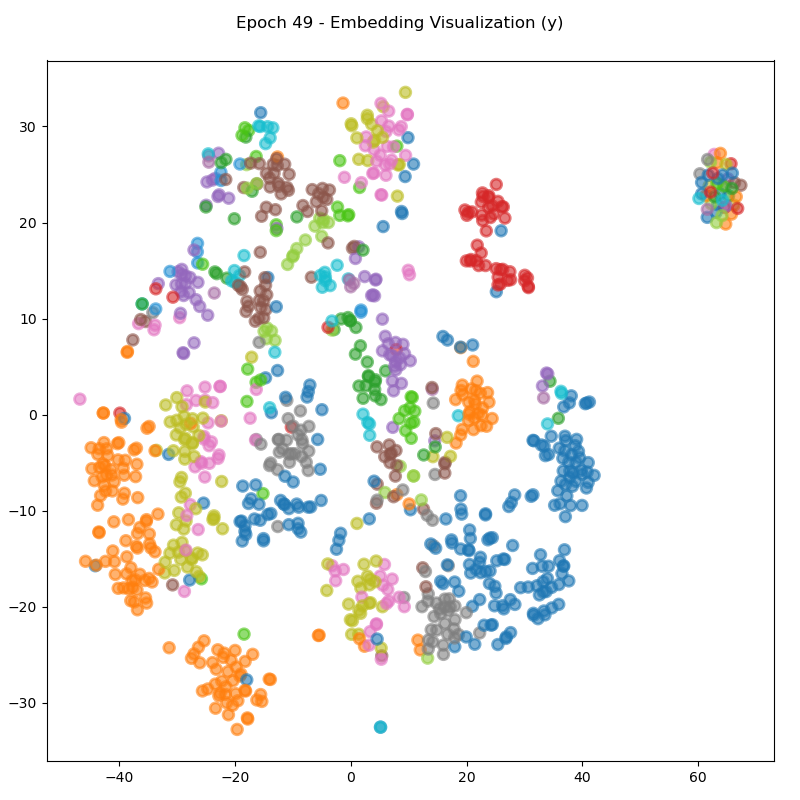
\includegraphics[width=0.23\columnwidth]{resources/visualization/combi_y.png}
}
\subfigure[$MGTCOM$ + $L_{\mathcal{T}}$]{
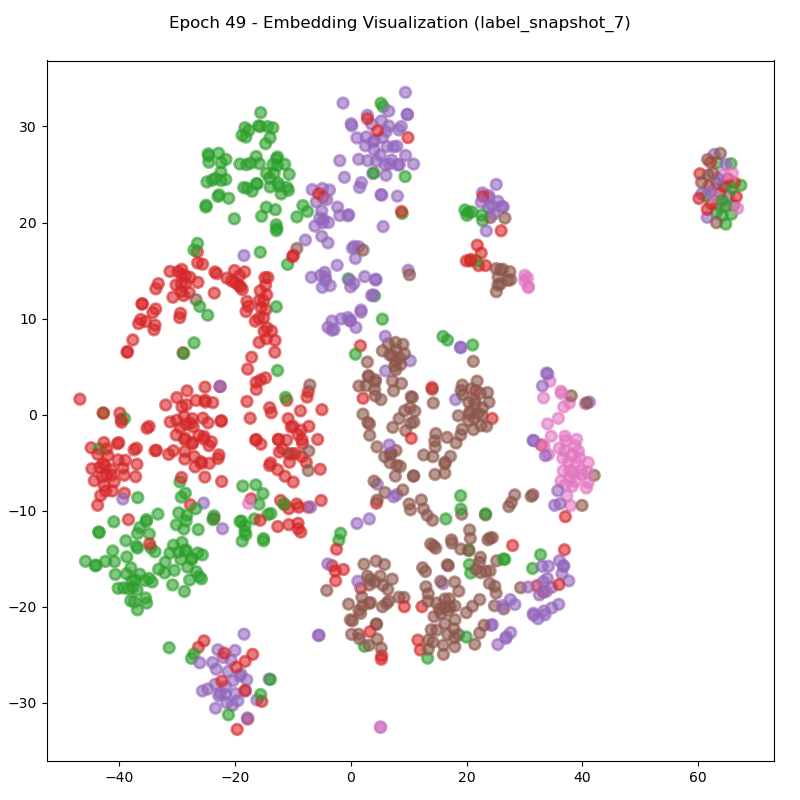
\includegraphics[width=0.23\columnwidth]{resources/visualization/combi_t.png}
}
\subfigure[$ComE$ + $L_y$]{
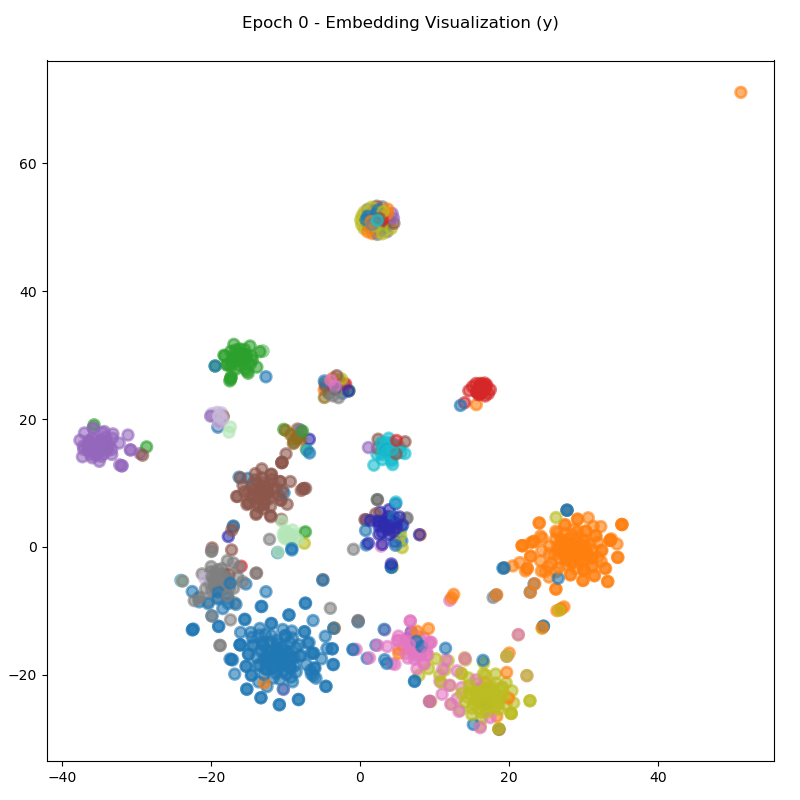
\includegraphics[width=0.23\columnwidth]{resources/visualization/come_y.png}
}
\subfigure[$ComE$ + $L_{\mathcal{T}}$]{
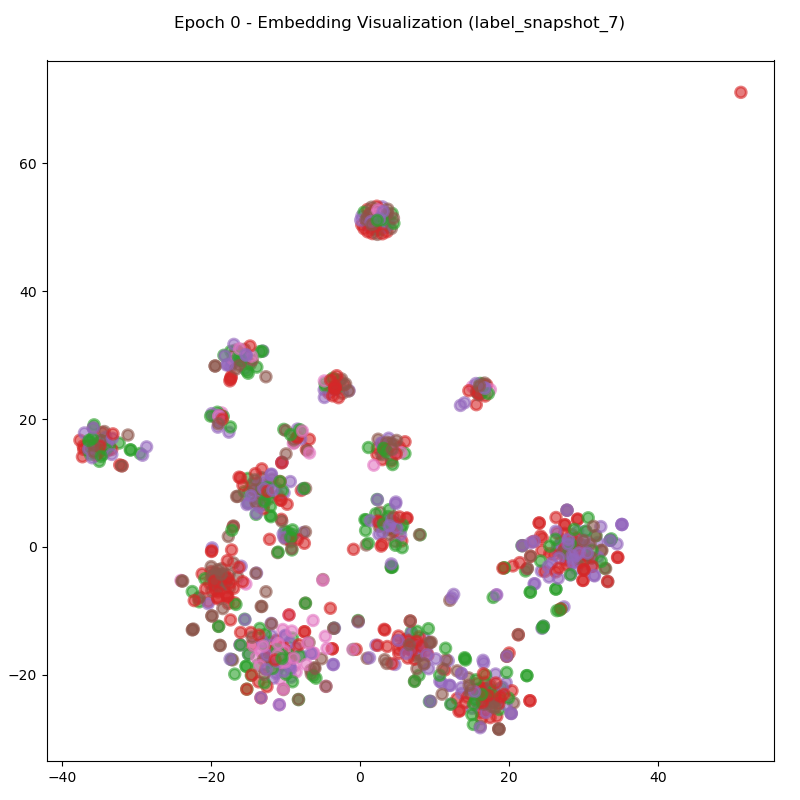
\includegraphics[width=0.23\columnwidth]{resources/visualization/come_t.png}
}\\

\centering
\subfigure[$Node2Vec$ + $L_y$]{
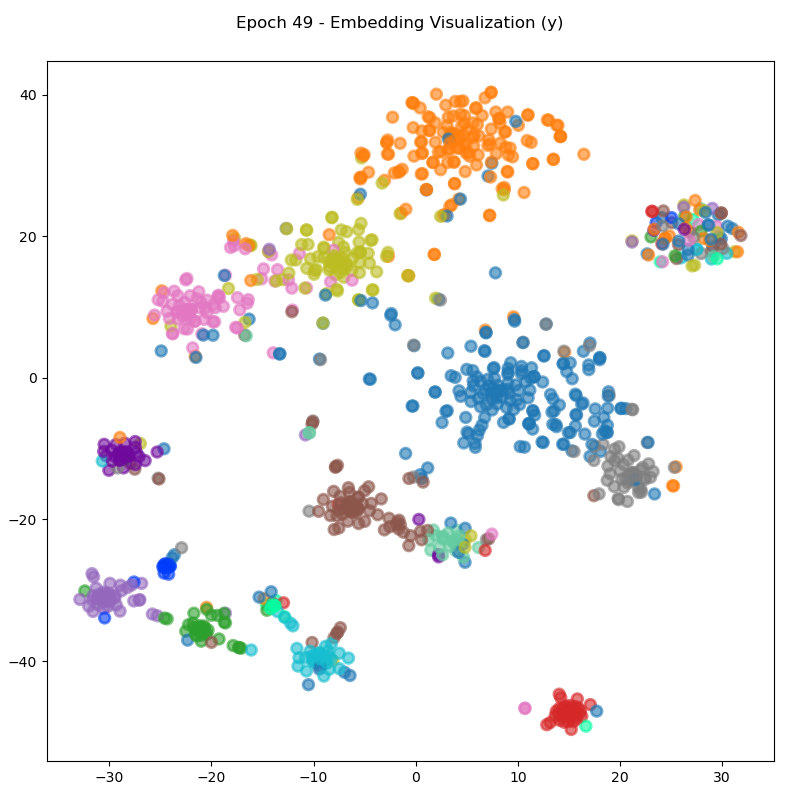
\includegraphics[width=0.23\columnwidth]{resources/visualization/n2v_y.png}
}
\subfigure[$Node2Vec$ + $L_{\mathcal{T}}$]{
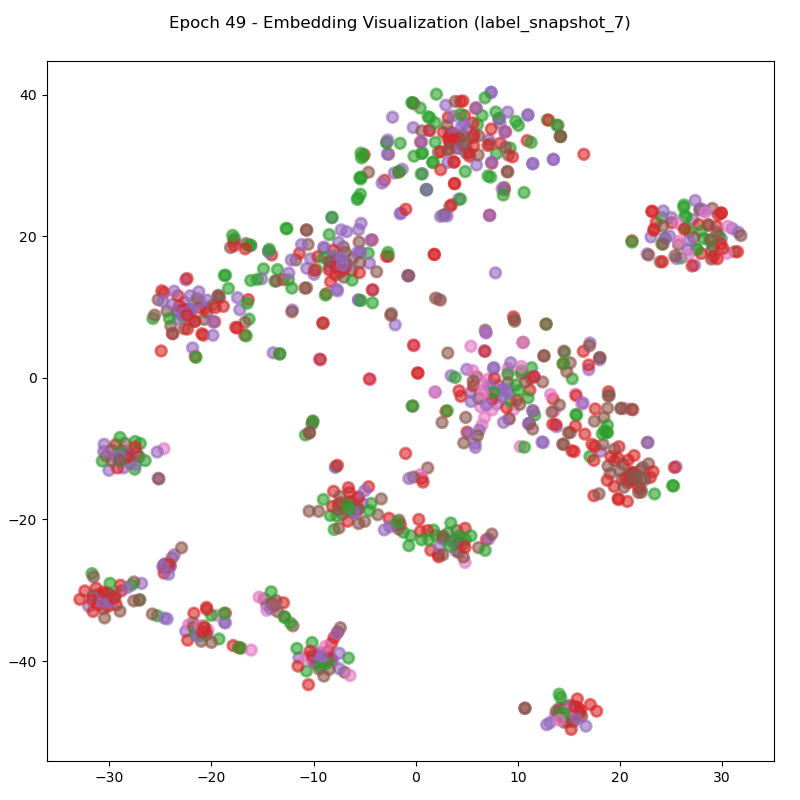
\includegraphics[width=0.23\columnwidth]{resources/visualization/n2v_t.png}
}
\subfigure[$CTDNE$ + $L_y$]{
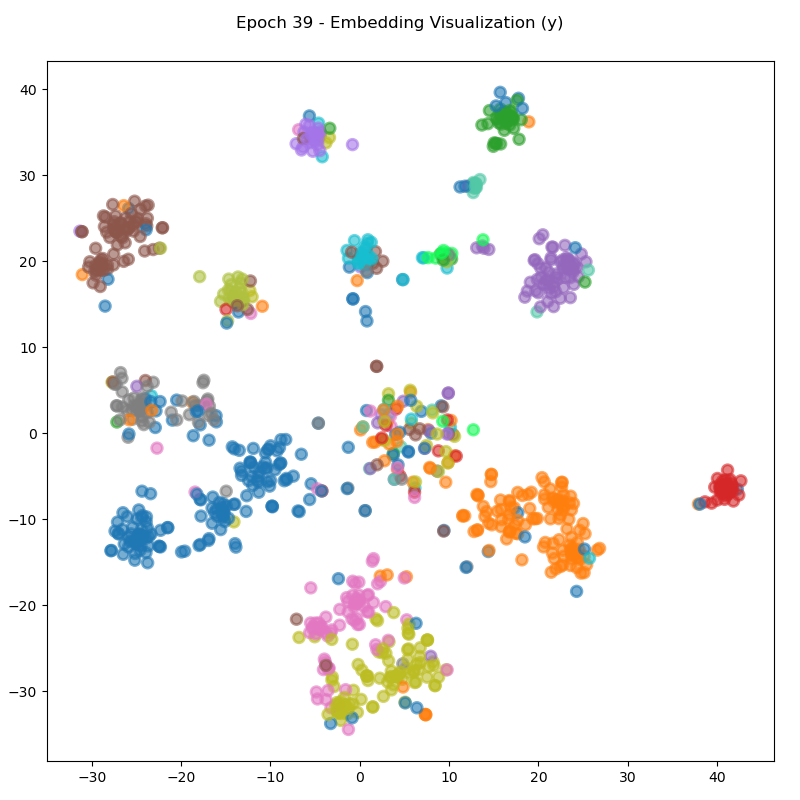
\includegraphics[width=0.23\columnwidth]{resources/visualization/ctdne_y.png} 
}
\subfigure[$CTDNE$ + $L_{\mathcal{T}}$]{
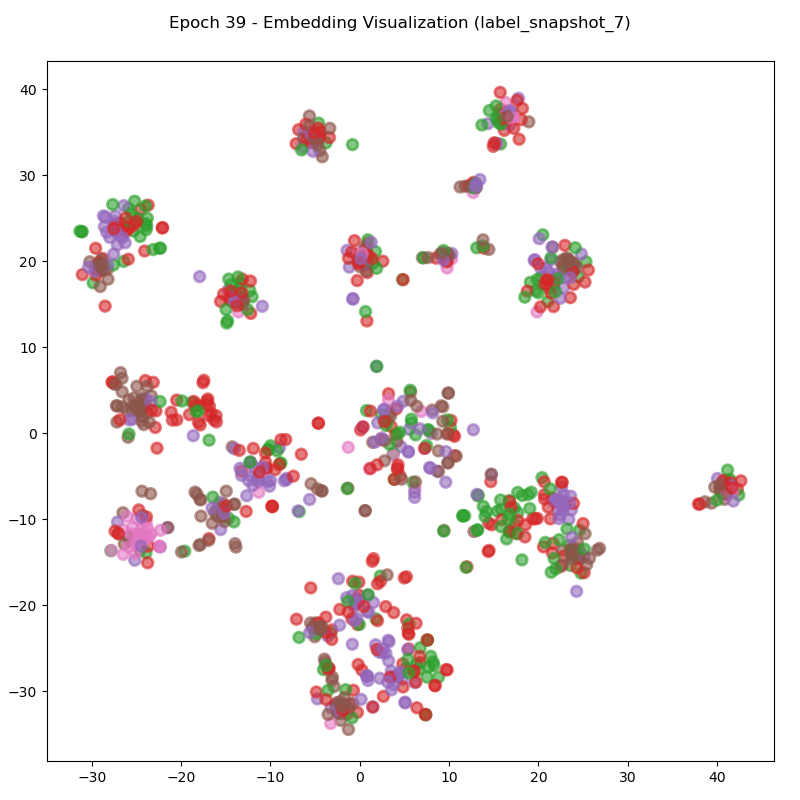
\includegraphics[width=0.23\columnwidth]{resources/visualization/ctdne_t.png}
}
\caption{Visualization of trained embedding against ground truth labels ($L_y$,  left) and timestamp labels ($L_{\mathcal{T}}$, right) for DBLP-HCN dataset.
(Note: The embeddings are calculated on the training dataset. Each of the plots contains a blob of nodes that have no edges in the training set due to the validation split. None of the methods is equipped to handle disconnected nodes.)
}
\label{fig:embeddings}
\end{figure*}    

We further compare $MGTCOM$ and the baseline models on the DBLP-HCN network.
We apply the T-SNE dimensionality reduction technique to visualize the trained node embeddings in 2D space colored by the ground truth label and the node timestamp (See \cref{fig:embeddings}).

Since in the DBLP-HCN dataset the timestamps are weakly correlated with its topology, we can see that topology-focused embedding (and community detection) methods such as ComE and Node2Vec do not capture temporal relations of nodes. On contrary, we observe distinct patterns emerge when looking at $MGTCOM$ generated embeddings for both of the labels.
%
Similar to that of $ComE$ the community structures are visible in the node embeddings though they are not as distinct.


%=====================================================================================
\section{Inference results}
Because the $MGTCOM$ model operates on sampled neighborhood subgraphs, in contrast to other methods it can operate in an inductive setting.
Meaning that it is not necessary to retrain the model to infer representation vectors for previously unseen nodes.

We evaluate the performance of $MGTCOM$ and its task-specific variants in inductive settings by controlling the ratio of nodes in the training set to the validation set.
The test set remains constant throughout the experiment to accurately assess performance on inferred nodes.
The relevant quality measures are computed exclusively on the test set and can be found in \cref{tab:results_inference}.

In \cref{fig:inference} we see the same measures plotted with the training ratio on the x-axis.
From \cref{fig:inference} (a) we observe that varying training set size does not affect link-prediction tasks as much as node classification tasks (b, c, d).
Throughout the measures, we can see that using only 75\% of the data does not substantially affect the results.
Interestingly, we observe that the variance on the temporal prediction task increases when more data is provided.

\begin{figure*}[t!]
\centering
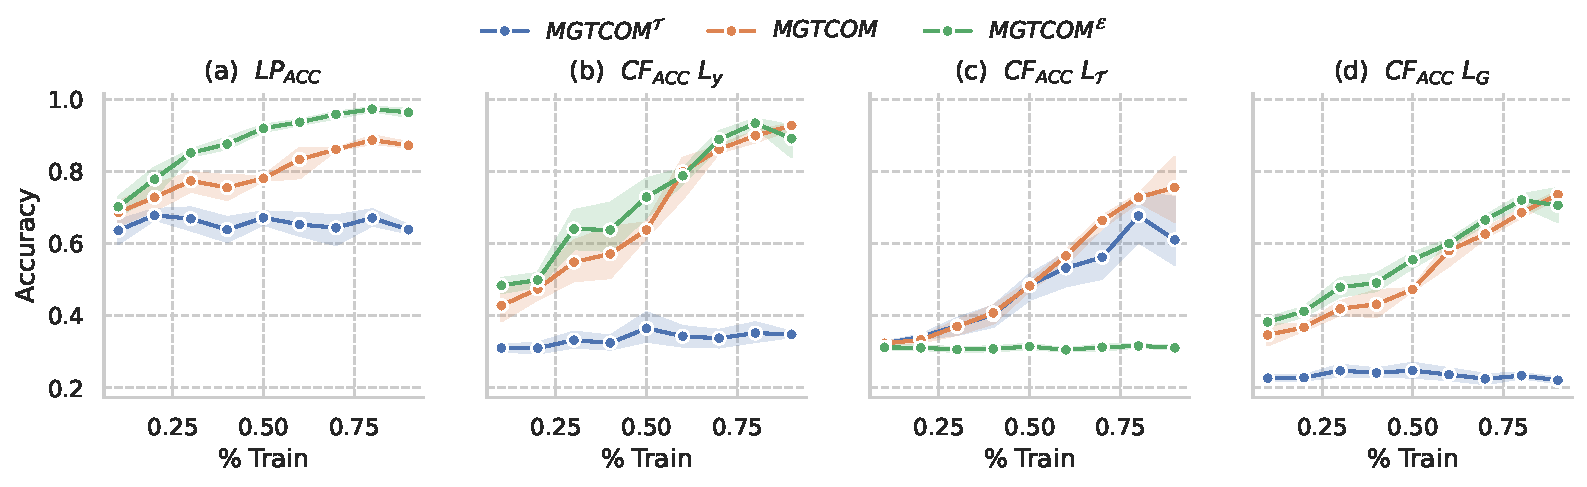
\includegraphics[width=\textwidth]{resources/figs/inference.pdf}
\caption{
    Visual comparison of different model variants in the inference-based setting. 
    Graph nodes are split into three disjointed sets (train, validation, and test).
    The metrics are measured while the training to validation ratio is varied. 
    The test set is set to 10\% of the nodes and is kept constant.
    The average metrics per data value are plotted along with their standard deviation.
}
\label{fig:inference}
\end{figure*}    
\begin{table*}[t!]
\centering
\caption{
    Comparison of different model variants in the inference-based setting. 
    Graph nodes are split into three disjointed sets (train, validation, and test).
    The metrics are measured while the training to validation ratio is varied. 
    The test set is set to 10\% of the nodes and is kept constant.
}
\label{tab:results_inference}
% \resizebox{\textwidth}{!}{
    \begin{tabular}{ll|ccccccccc}
    \toprule
     \textbf{Model}                      & \textbf{\% Train} &            10\% &            20\% &            30\% &            40\% &            50\% &            60\% &            70\% &            80\% &            90\% \\ 
    \midrule
$MGTCOM$ 
                       & $LP_{ACC}$ &  0.686 &  0.728 &  0.774 &  0.755 &  0.780 &  0.833 &  0.861 &  0.887 &  0.872 \\
                       & $CF_{ACC}$ $L_y$ &  0.428 &  0.474 &  0.548 &  0.571 &  0.638 &  0.799 &  0.861 &  0.899 &  0.927 \\
                       & $CF_{ACC}$ $L_\mathcal{T}$ &  0.323 &  0.333 &  0.370 &  0.408 &  0.483 &  0.566 &  0.664 &  0.728 &  0.755 \\
                       & $CF_{ACC}$ $L_G$ &  0.347 &  0.368 &  0.419 &  0.432 &  0.473 &  0.580 &  0.626 &  0.685 &  0.736 \\ \midrule
$MGTCOM^{\mathcal{E}}$ 
                       & $LP_{ACC}$ &  0.702 &  0.778 &  0.851 &  0.876 &  0.919 &  0.936 &  0.958 &  0.972 &  0.963 \\
                       & $CF_{ACC}$ $L_y$ &  0.484 &  0.499 &  0.640 &  0.637 &  0.729 &  0.788 &  0.888 &  0.933 &  0.891 \\
                       & $CF_{ACC}$ $L_\mathcal{T}$ &  0.312 &  0.311 &  0.306 &  0.308 &  0.314 &  0.305 &  0.312 &  0.316 &  0.311 \\
                       & $CF_{ACC}$ $L_G$ &  0.382 &  0.412 &  0.479 &  0.491 &  0.555 &  0.600 &  0.665 &  0.721 &  0.706 \\ \midrule
$MGTCOM^{\mathcal{T}}$ 
                       & $LP_{ACC}$ &  0.636 &  0.678 &  0.669 &  0.639 &  0.671 &  0.653 &  0.644 &  0.671 &  0.638 \\
                       & $CF_{ACC}$ $L_y$ &  0.310 &  0.310 &  0.332 &  0.324 &  0.365 &  0.343 &  0.337 &  0.352 &  0.348 \\
                       & $CF_{ACC}$ $L_\mathcal{T}$ &  0.323 &  0.341 &  0.372 &  0.403 &  0.485 &  0.532 &  0.562 &  0.677 &  0.610 \\
                       & $CF_{ACC}$ $L_G$ &  0.227 &  0.228 &  0.248 &  0.242 &  0.248 &  0.237 &  0.225 &  0.234 &  0.221 \\
    \bottomrule
    \end{tabular}

% }
\end{table*}


%=====================================================================================
\section{Learnable parameter reduction}
An important goal of our work is to prove that inductive-based community detection is feasible.
We address the structural similarity bias found in many unsupervised inductive algorithms by introducing a custom loss and sampling methodology in \cref{sec:obj_fn}.
While our model still utilizes embeddings to address the incompleteness constraints, we show in \cref{sec:abl:aux_emb} that importance-based pruning is an effective optimization to keep the model scalable.

As result, our model takes advantage of the scalability of inductive representation learning methods.
In \cref{tab:params} we compare the parameter count of the $MGTCOM$ model to the node2vec model which directly learns node embeddings.
Overall $MGTCOM$ has fewer parameters since the model size is bound by meta-topology.
In highly heterogeneous graphs such as the ICEWS dataset, the number of parameters may become larger than expected.
Specifically, the number of parameters is proportional to $|\mathcal{A}| + |\mathcal{R}|$.
For exact analysis on the number of learnable parameters the model uses, we refer the reader to \cref{sec:exact_params}. 

\begin{table}[ht!]
\centering
\caption{
    Parameter count comparison between node2vec and the $MGTCOM$ model.
    \label{tab:params}
}
% \resizebox{\columnwidth}{!}{
\small
\begin{tabular}{l|ll}
    \hline
    Dataset & node2vec  & $MGTCOM$  \\ \hline
    DBLP    & 683,968   & 173,910   \\
    ICEWS   & 669,632   & 1,072,302 \\
    IMDB    & 867,840   & 170,846   \\
    SDS     & 5,979,712 & 231,282   \\
    Cora    & 173,312   & 136,390   \\ \hline
\end{tabular}
% }
\end{table}
\chapter{Ablation study} \label{sec:ablation}
In this section, we investigate the sensitivity of our model to the described design choices and hyperparameter values.
Throughout the experiments, we keep the same base parameters as described in the experimental setup.
Similarly, the DBLP dataset is used throughout as it provides a wide range of features suitable for the evaluation of all supported tasks.

% ====================================================
\section{Auxiliary Embedding Ratio} \label{sec:abl:aux_emb}
To address the incompleteness constraints, $MGTCOM$ introduces auxiliary embeddings for nodes without features.
Zero-vector features are used for nodes that are unseen during training and don't have their own feature vector to encourage its inference from neighboring nodes.
While doing this introduces performance benefits, for large datasets it may not be possible to store the auxiliary embeddings in memory.

We define a procedure to work around this scaling issue by noting that embeddings only need to be constructed for a fraction of the most important nodes.
This is due to scaling laws applicable to most real-world networks.
Specifically, in this experiment, we sort all the nodes without features by their degree and use a fraction of the highest degree nodes for auxiliary embeddings. Other nodes are given a zero-vector upon inference.

\begin{figure}[ht]
\centering

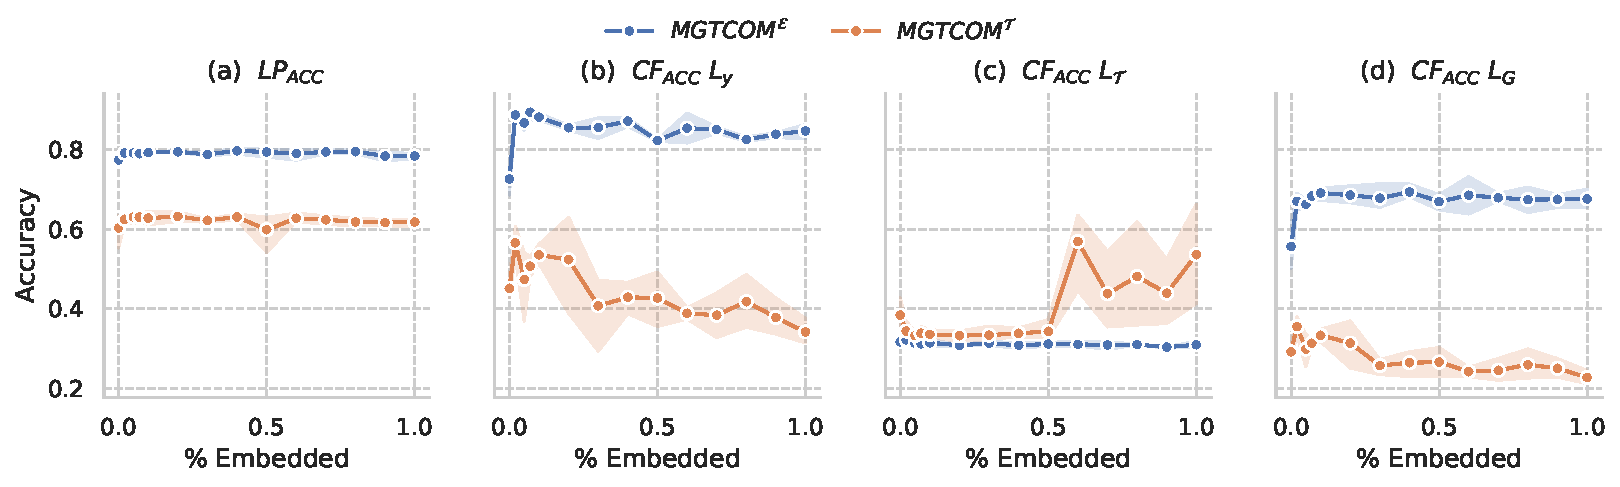
\includegraphics[width=\columnwidth]{resources/figs/embed_ratio.pdf}

\caption{
Performance results for topological $MGTCOM^{\mathcal{E}}$ and temporal $MGTCOM^{\mathcal{T}}$ models on various tasks where the ratio of auxiliary embedded nodes varies.
}
\label{fig:abl_embed_ratio}
\end{figure}
In \cref{fig:abl_embed_ratio} we see the results of the tasks specific models when the auxiliary ratio is varied.
From figure (a) we can observe that while auxiliary embeddings don't have a large influence during link prediction, they are in fact necessary on prediction tasks as figures (b), (c), and (d) indicate.
It can be rightfully deduced that embeddings are necessary for temporal tasks (figure (c)) since topology and content-based features are weakly correlated with temporal features.

% ====================================================
\section{Meta-topological features}
Meta-topological features are an important part of multimodal graphs.
In this experiment, we aim to determine the importance of meta-topology in our evaluation setting.
We evaluate the performance measures on heterogeneous and homogeneous variants of the DBLP dataset.
By varying convolutional layers between Heterogeneous Graph Transformer and GraphSAGE \cite{csirosdata61StargazersStellargraphStellargraph2018} (each edge type has a separate set of weights), we additionally aim to determine the importance of meta-topology-based attention used during the aggregation step.

\begin{figure}[ht]
\centering

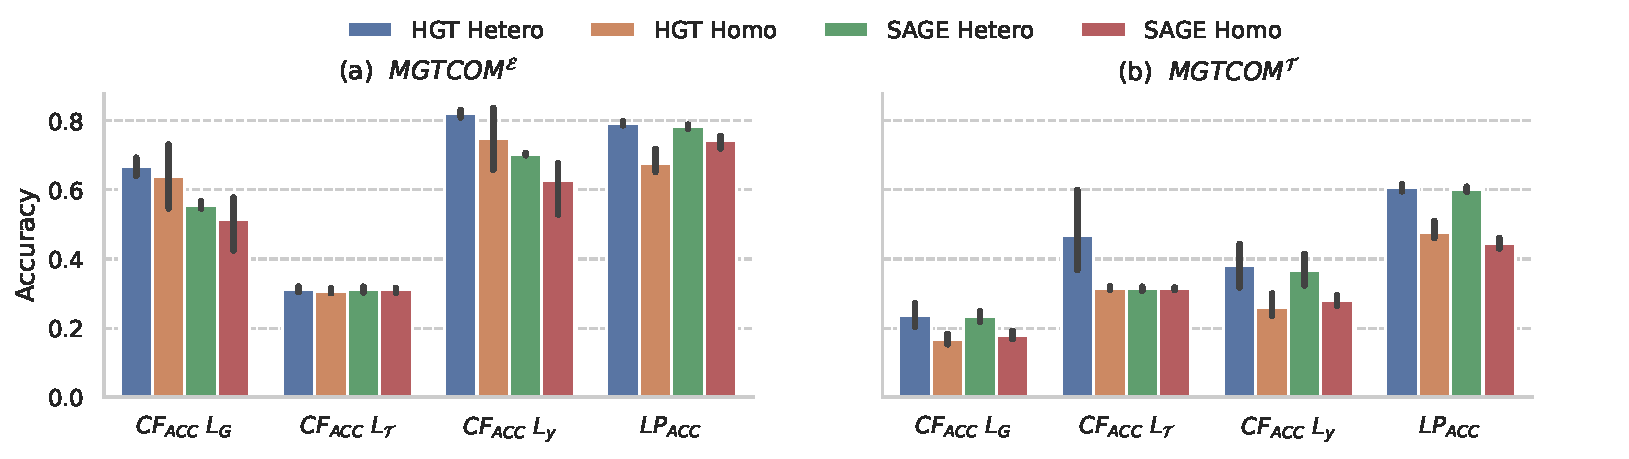
\includegraphics[width=\columnwidth]{resources/figs/abl_meta.pdf}

\caption{
Performance results for (a) topological $MGTCOM^{\mathcal{E}}$ and (b) temporal $MGTCOM^{\mathcal{T}}$ models, on prediction tasks for heterogeneous and homogeneous variants of the DBLP dataset.
To determine the importance of meta-topological attention we vary the convolutional layers HGT and GraphSAGE (which is adopted for heterogeneous graphs).
}
\label{fig:ablation_meta}
\end{figure}

Overall in \cref{fig:ablation_meta} we see that the addition of meta-topological features has a positive effect on the classification performance of both topological as well as temporal models. 
This effect is especially pronounced on link prediction and topology-based classification tasks for the temporal model. 
The cause for this may be that while topological features are not provided during training, meta-topology still conveys enough information about the topology.

From the results, we see that meta-topology-based attention yields benefits in classification performance in contrast to naive aggregation techniques (improvement by ~10\%).

% ====================================================
\section{Trade-off Parameter} \label{sec:abl:aux_emb}
During analysis the trade-off parameters ($\beta^{\mathcal{E}}$, $\beta^{\mathcal{T}}$, $\beta^{\mathcal{C}}$) are used to guide the trained embeddings to favor specific tasks.
In this experiment, we explore the trade-off between temporal and topological tasks by varying value of $\beta^{\mathcal{E}}$, $\beta^{\mathcal{T}}$ while setting the constraint $1 = \beta^{\mathcal{E}}$ + $\beta^{\mathcal{T}}$. 
The clustering weight parameter $\beta^{\mathcal{C}}$ remains constant throughout as described in \cref{sec:exp_setup}.

In \cref{fig:abl_beta} (a) we can see an almost linear correlation between link prediction accuracy and the topological weight parameter $\beta^{\mathcal{E}}$.
On the other hand, in figures (b) and (d) we see a more logarithmic curve for topology correlated classification measures.
The most interesting takeaway is that while variance is quite high on the temporal classification task, its curve peaks at a value of 0.5.
In further work, it may be worth exploring this phenomenon in more detail. 
The most probable assumption would be that the temporal model still benefits from the fact that temporal features are weakly correlated with the topology.

\begin{figure}[ht!]
\centering

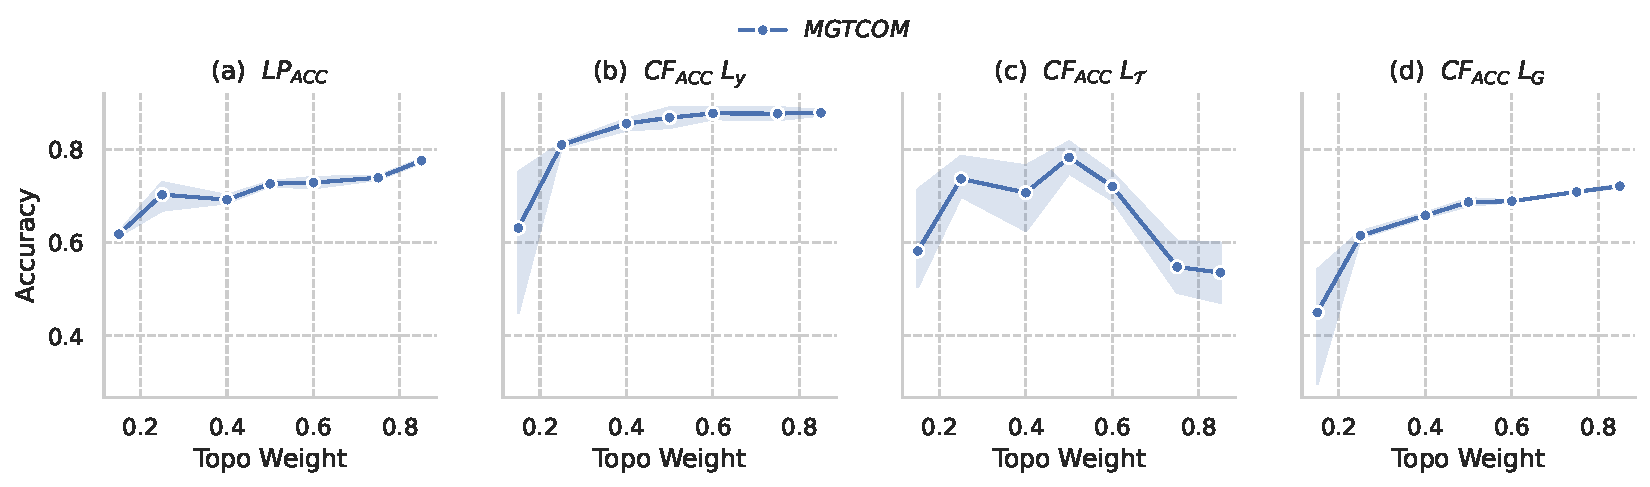
\includegraphics[width=\columnwidth]{resources/figs/abl_beta_topo.pdf}

\caption{
Performance of $MGTCOM$ model while varying topological loss weight parameter $\beta^{\mathcal{T}}$ under $1 = \beta^{\mathcal{E}}$ + $\beta^{\mathcal{T}}$ contraint.
}
\label{fig:abl_beta}
\end{figure}

% ====================================================
\section{Initial $K$ sensitivity}
In this section evaluate the sensitivity of the clustering results to the initial $K$ value selection.
While our method does not require setting the cluster to count $K$, it can still be set to find more accurate initial clustering, and help DPMM avoid local minima.
Specifically, we have varied the initial cluster count (init $K$) used for k-means initialization while keeping all other parameters fixed.

\begin{figure}[ht]
\centering

\subfigure[]{
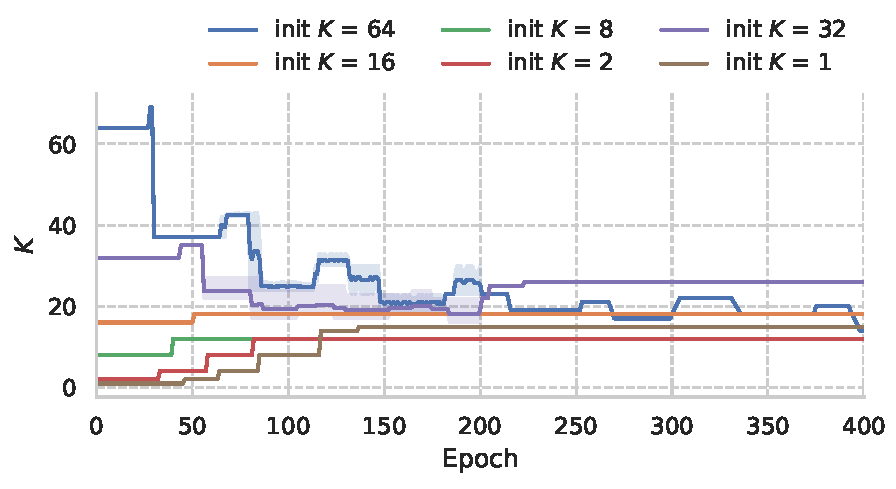
\includegraphics[width=0.48\textwidth]{resources/figs/abl_initk_k.pdf}
}
\subfigure[]{
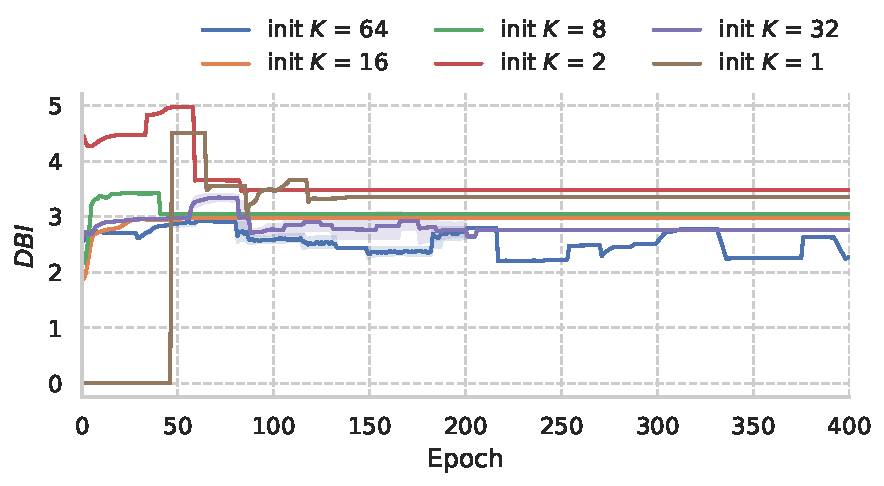
\includegraphics[width=0.48\textwidth]{resources/figs/abl_initk_dbi.pdf}
}

\caption{
(a) and (b): Cluster count progression during DPMM clustering given an initial cluster count (init $K$). The clustering is done on pre-trained $MGTCOM$ embeddings for the DBLP dataset.
}
\label{fig:ablation_k}
\end{figure}

In \cref{fig:ablation_k} (a) we see that despite varying starting values, all the runs converge at 12-18 cluster range.
Having a value that strongly deviates from the "optimal" cluster count causes a slower convergence since more split/merge operations are required.
We can see a similar pattern in the measured Davies-Bouldin index in \cref{fig:ablation_meta} (b).

% ====================================================
\section{Hyperparameter sensitivity} \label{sec:abl:hyperparam}
\begin{figure}[ht!]
\centering
\subfigure[]{
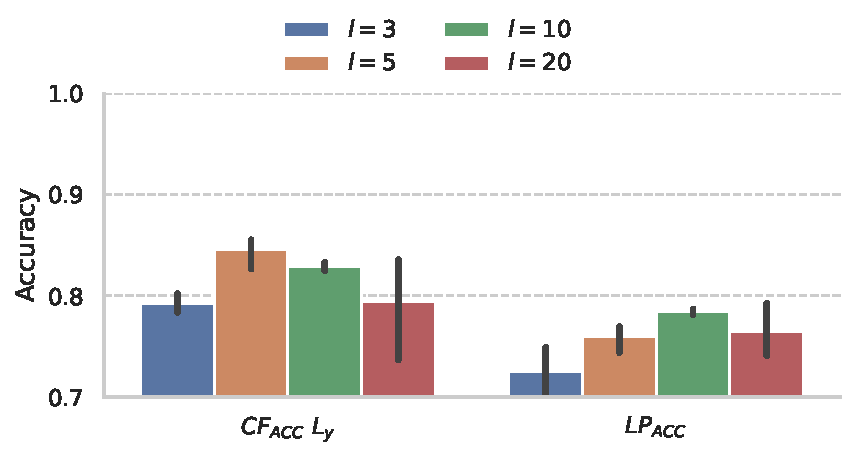
\includegraphics[width=0.47\textwidth]{resources/figs/tune_topo_rw_ctx.pdf}
}\quad
\subfigure[]{
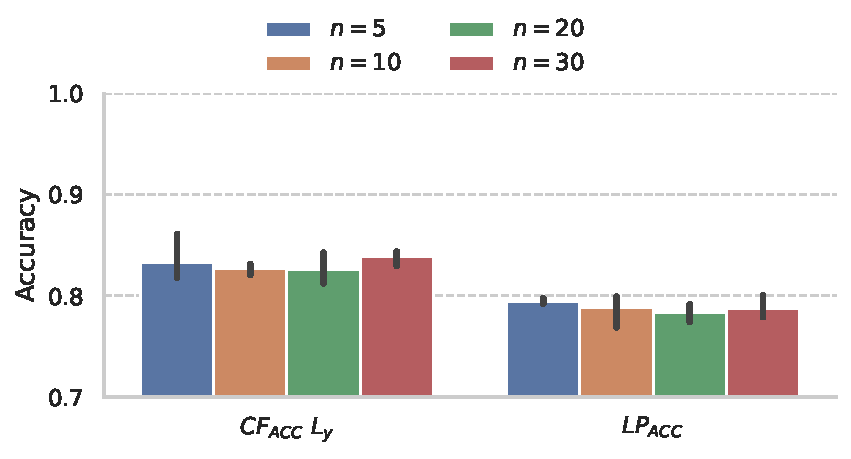
\includegraphics[width=0.47\textwidth]{resources/figs/tune_topo_rw_nwalks.pdf}
}\quad
\subfigure[]{
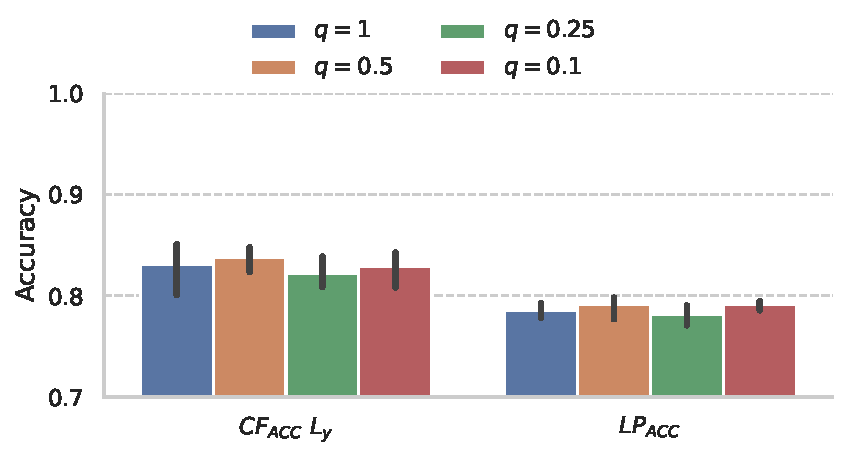
\includegraphics[width=0.47\textwidth]{resources/figs/tune_topo_rw_q.pdf}
}\quad
\caption{
Performance of $MGTCOM^{\mathcal{E}}$ model with varying (a) random walks length $l$, (b) number of random walks per node $n$, and (c) the exploration trade-off parameter $q$.
}
\label{fig:hyp_rw_topo}
\end{figure}    

In this part, the sensitivity of other hyperparameters on the model performance is discussed.
%
The node2vec random walk algorithm used for the topological task relies on parameters such as walk length $l$, the number of random walks $n$ for each node, and the exploration trade-off parameter $q$.
In \cref{fig:hyp_rw_topo} we see that while the choice of random walk length has a significant impact on link-prediction and classification performance (a), the model is not as sensitive to the other parameters.
A surprising observation is that the trade-off parameter does not significantly affect the productivity accuracy of ground communities ($CF_{ACC}$ $L_y$).
A possible explanation for this may be the fact that we use both random walk and neighborhood sampling algorithms making the trade-off ineffective.

\begin{figure}[ht!]
\centering
\subfigure[]{
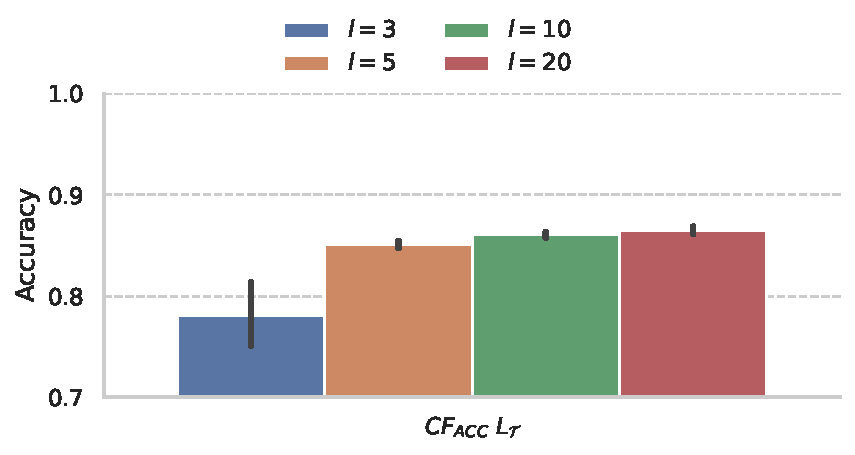
\includegraphics[width=0.47\textwidth]{resources/figs/tune_tempo_rw_ctx.pdf}
}\quad
\subfigure[]{
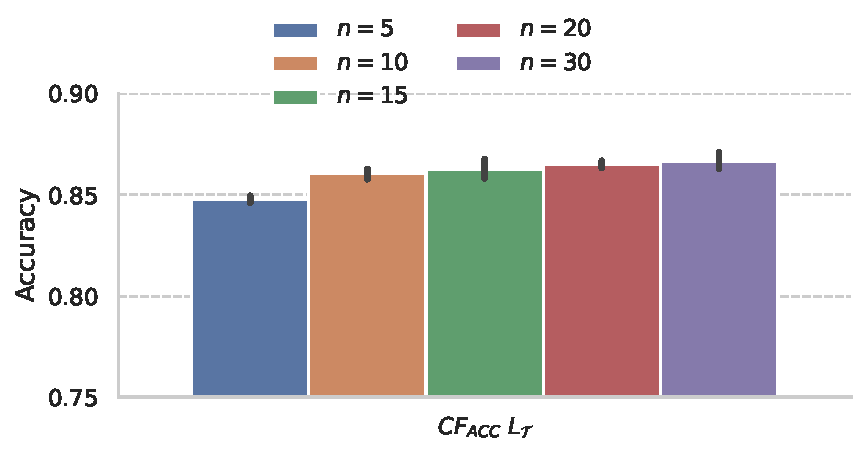
\includegraphics[width=0.47\textwidth]{resources/figs/tune_tempo_rw_nwalks.pdf}
}\quad
\caption{
Performance of $MGTCOM^{\mathcal{T}}$ model with varying (a) random walks length $l$ and (b) number of random walks per node $n$.
}
\label{fig:hyp_rw_tempo}
\end{figure}    

The ballroom walk algorithm introduced in \cref{sec:tempo_sampling} similarly relies on the hyperparameters walk length $l$ and the number of random walks started for each node $n$, though they serve a different purpose.
Increasing either the $l$ or the $n$ parameter only marginally increases the models performance at timestamp prediction (See \cref{fig:hyp_rw_tempo}).
For both parameters, there is a positive correlation between performance and an increase in the receptive field. 

\begin{figure}[ht!]
\centering
\subfigure[]{
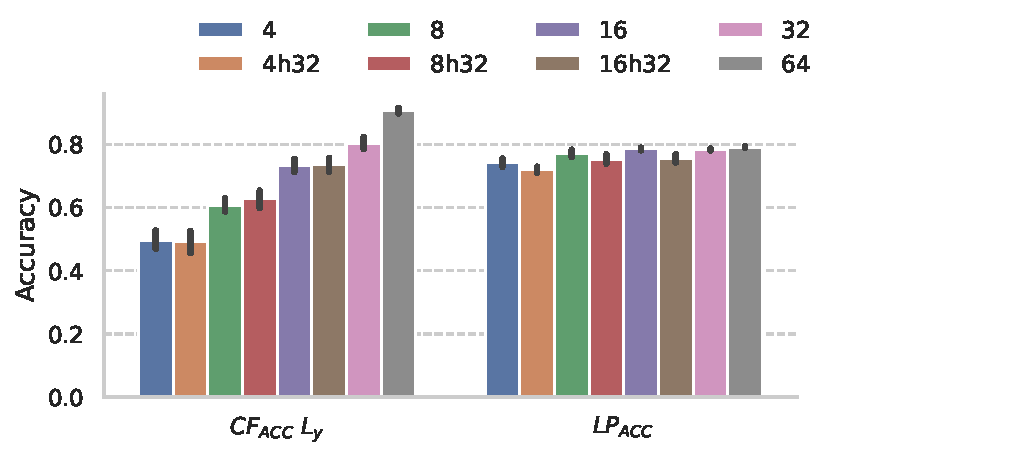
\includegraphics[width=0.47\textwidth]{resources/figs/tune_topo_reprdim.pdf}
}\quad
\subfigure[]{
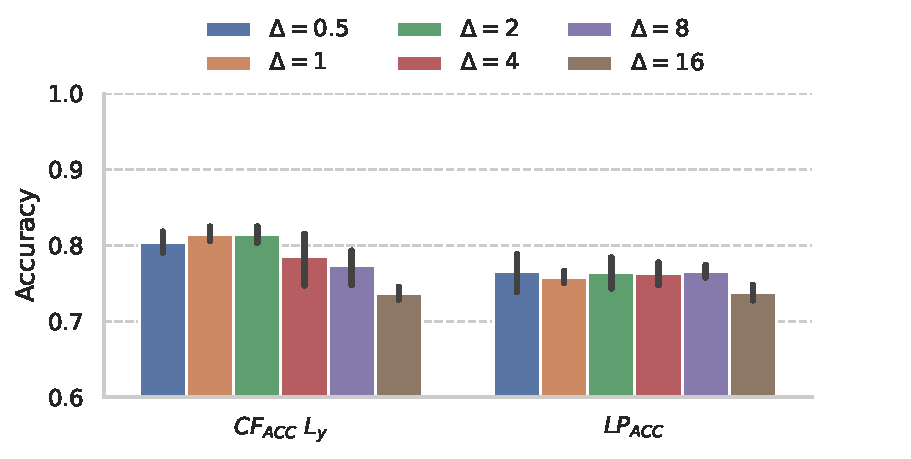
\includegraphics[width=0.47\textwidth]{resources/figs/tune_topo_margin.pdf}
}\quad
\subfigure[]{
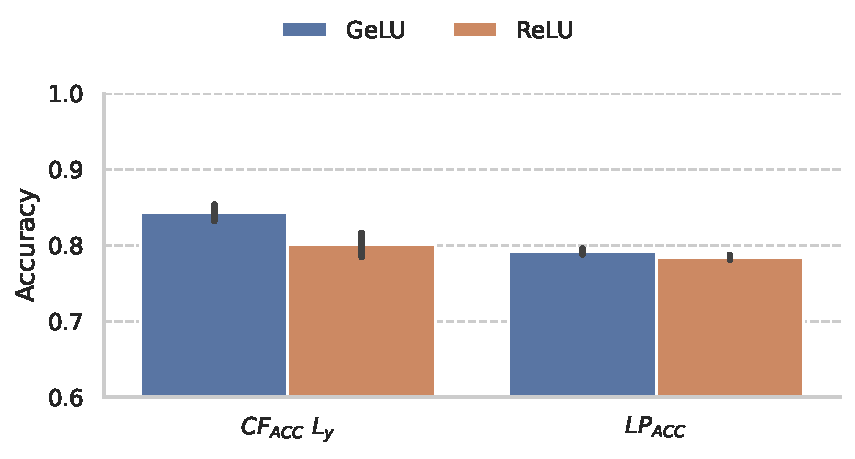
\includegraphics[width=0.46\textwidth]{resources/figs/tune_topo_activation.pdf}
}\quad
\caption{
Performance of $MGTCOM^{\mathcal{E}}$ model with varying (a) representation dimension $d$, (b) the margin ($\Delta$) parameter for the hinge loss, and (c) activation function.
}
\label{fig:hyp_rw_repr}
\end{figure}    

The most sensitive/important parameter for our model is the representation dimension size $d$.
In \cref{fig:hyp_rw_repr} (a) we plot the predictive performance of the topological model while varying the model representation dimension $d$ and the hidden representation dimension $h$ used in in-between layers of graph convolution.
The classification performance seems to benefit the most from a larger $d$, while link-prediction only sees a marginal improvement.
Moreover having hidden dimension size deviate from the representation dimension only seems to degrade the model performance.

In \cref{fig:hyp_rw_repr} (b) we vary the margin parameter of hinge loss. 
It is conventional to use $\Delta = 1$ if the similarity is bounded (as is in our case), therefore we can see the model performance degrade as the margin exceeds this threshold.
Increasing loss beyond $1$ amplifies the relative relevance of small loss samples, which in turn makes the model more prone to noise.

While constructing the network we found that the choice of activation function noticeably affects the model performance. 
Choosing GeLU over ReLU activation speeds up model convergence and gains a noticeable edge in classification tasks (See \cref{fig:hyp_rw_repr} (c)).

\begin{figure}[]
\centering

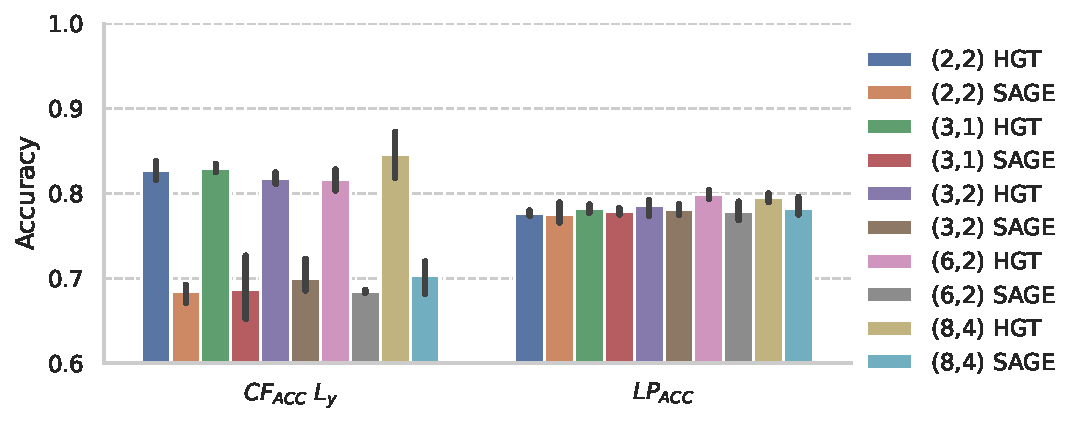
\includegraphics[width=0.6\columnwidth]{resources/figs/tune_topo_neigh.pdf}

\caption{
Performance of $MGTCOM^{\mathcal{E}}$ model with varying convolution layers. 
We vary the architecture by switching between Heterogeneous Graph Transformer (HGT) and Heterogenous GraphSAGE convolutional layers.
Similarly, we also modify the neighborhood size of each node within the two-layer convolution setup. 
Format $(x, y)$ represents the number of neighbors per node in the first ($x$) and second ($y$) layer respectively.
}
\label{fig:hyp_neigh}
\end{figure}

In \cref{fig:hyp_neigh} we vary the convolution architecture of the topological model and measure the resulting test performance.
As observed earlier HGT convolutional layers perform better since they introduce meta-topology-based attention. 
Varying the layer neighborhood size does not seem to affect the performance substantially, except for the fact that computed performance measures during training are a lot smoother throughout.

\begin{figure}[]
\centering
\subfigure[]{
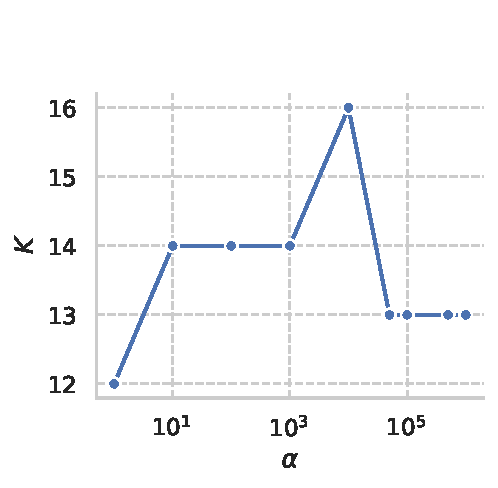
\includegraphics[width=0.3\textwidth]{resources/figs/cluster_alpha.pdf}
}\quad
\subfigure[]{
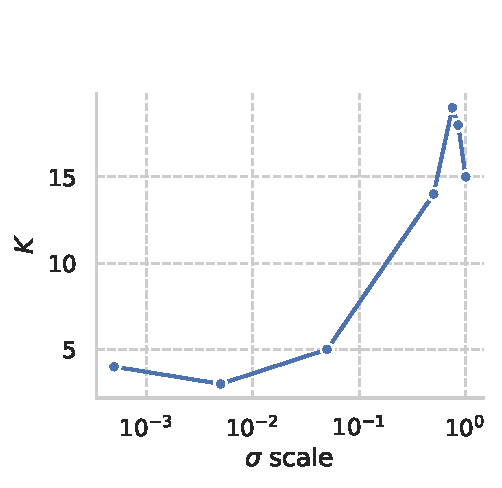
\includegraphics[width=0.3\textwidth]{resources/figs/cluster_sigma_scale.pdf}
}\quad \\
\subfigure[]{
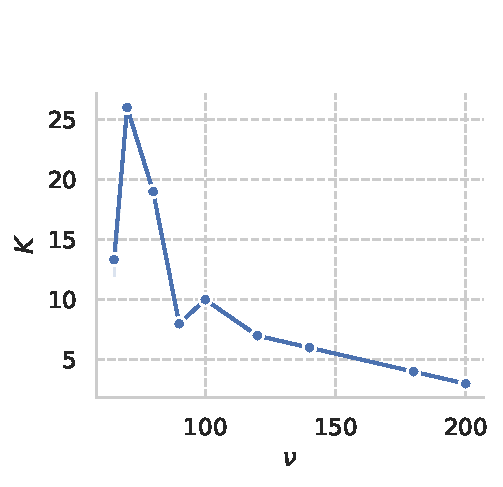
\includegraphics[width=0.3\textwidth]{resources/figs/cluster_nu.pdf}
}\quad
\subfigure[]{
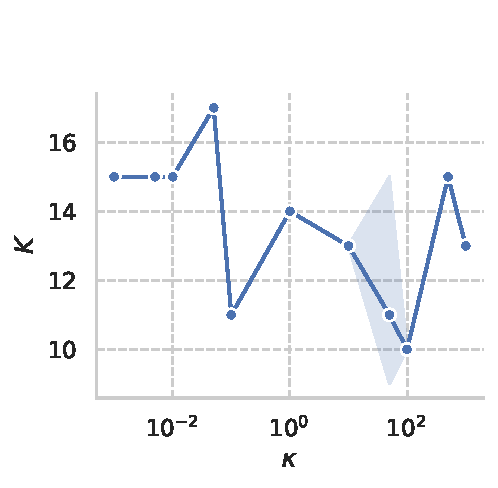
\includegraphics[width=0.3\textwidth]{resources/figs/cluster_kappa.pdf}
}\quad
\caption{
    Sensitivity of the resulting cluster count $K$ on the DPMM prior parameters (a) $\alpha$ the cluster concentration parameter, (b) the $\sigma$ scale parameter influencing the covariance of prior, (c) $\nu$ the degrees of freedom parameter for the Wishart prior distribution, and (d) $\kappa$ the concentration parameter of the Wishart prior distribution.
}
\label{fig:hyp_cluster}
\end{figure}

Finally, in \cref{fig:hyp_cluster} we analyze the sensitivity of the resulting cluster count to the chosen prior parameters for the DPMM algorithm.
We notice that the $\sigma$ scale and $\nu$ parameters have a linear correlation with the resulting number of clusters.
The $\sigma$ scale parameter influences the data-bound $W$ hyperparameter and is to be expected to have a great impact.
A larger prior covariance corresponds to a larger probability that any of the clusters are drawn from it and therefore results in a larger number of clusters.
On the contrary, a larger degree of freedom requires a larger amount of samples per cluster, therefore reducing the probability of smaller clusters.
We see a more noisy pattern from $\alpha$ and $\kappa$ concentration hyperparameters as they are not data-bound and are less effective when their value is much smaller than the total number of data points $N$.



\chapter{Case study: Social Distancing Students dataset} \label{sec:case_study}
The Social Distancing Students dataset explores dutch public sentiment on governmental COVID-19 measures on Twitter based on data between February to September 2020 \cite{wangPublicSentimentGovernmental2020}.
Public sentiment is an important measure to consider before implementing certain measures or policies as it may influence compliance or cause protests.

The dataset consists of a tweet network encapsulating tweet, retweet, quote, and mention relations and a follower network modeling dynamics of the Twitter social network platform.
The network is constructed by gathering tweets matching a predefined set of keywords related to the COVID-19 crisis.
The follower network is constructed central to the users related to the tweets.
Following the work in the original paper, the dataset contains sentiment analysis labels indicating whether a tweet is in support or rejection of contemporary social distancing policies.

For this case study we have trained the $MGTCOM$ model on the dataset using the same parameters as described in the evaluation (\cref{sec:exp_setup}).
In the following steps, we use the dataset as well as training results to explore the patterns found in the data.
Additionally, we attempt to explain the learned features and communities based on the patterns seen in the data they capture.

\begin{figure}[ht!]
\centering
\subfigure[]{
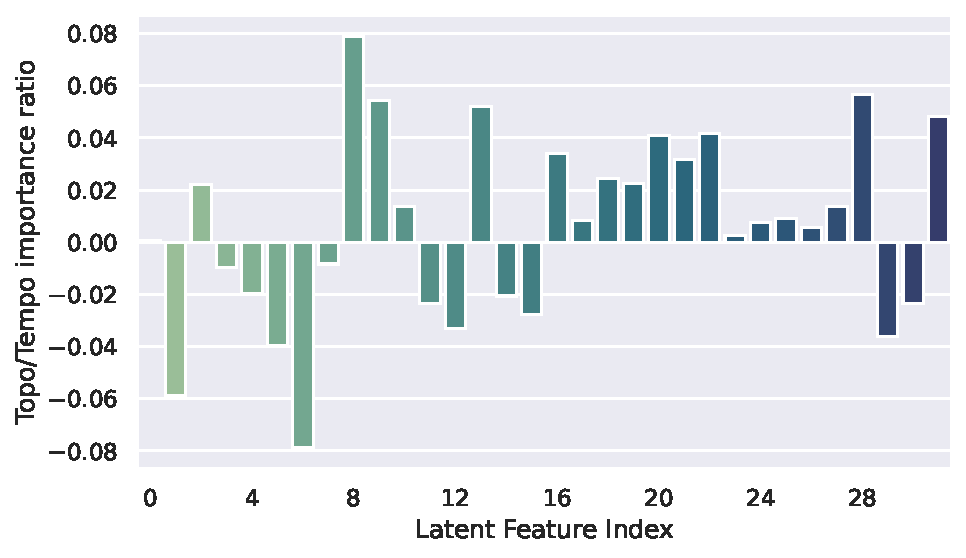
\includegraphics[width=0.47\textwidth]{resources/figs/case_study/02_att_topo_v_tempo.pdf}
}\quad
\subfigure[]{
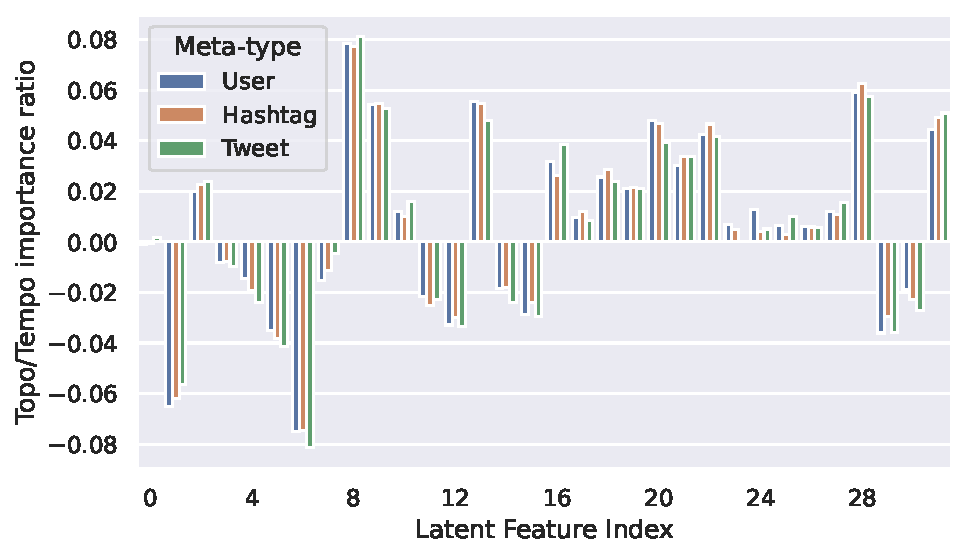
\includegraphics[width=0.47\textwidth]{resources/figs/case_study/03_att_topo_v_tempo_type.pdf}
}\quad
\caption{
    Given a latent feature vector ($d = 32$), for each feature, we plot attention averaged over the whole dataset.
    A positive value means the feature is more important for topological tasks, while a negative value means it is more important for temporal tasks.
    In plot (b) we similarly visualize the attention averaged over data points while grouped by node type.
}
\label{fig:cs_att_ratio}
\end{figure}

In the first step of our analysis, we focus on the relative importance of various embeddings features given their task-specific attention weight.
In \cref{fig:cs_att_ratio} we plot the attention ratio, which is computed as the mean difference between the topological and temporal feature-wise attention ($ATT^{\mathcal{E}} - ATT^{\mathcal{T}}$).
Since, the attention is computed per node, in figure (b) we plot the attention ratio grouped by node type.
While on the feature level a clear distinction is seen where features are more important for either task, we can see that attention between different types doesn't deviate much from the mean.
This is not unexpected as the attention is not parameterized by meta-topology, as it is rather implicitly encoded in the primary embedding vector.

In \cref{fig:cs_tempo_feat_hist} we visualize a temporal histogram for top nodes given individual features that have a higher average temporal attention.
Because our distance measure is based on inner-product, the selection of top nodes works by simply sorting node embeddings by the selected feature in descending order.
In almost all the subplots we see pronounced peaks at certain timestamps indicating that the latent features capture certain temporal patterns within the data.
Since many features capture the peaks during mid-October it is fair to assume that those tweets have certain distinct underlying properties. 
As a baseline, we plot the general tweet distribution over time in \cref{fig:cs_ts_dist} to compare the peaks in feature histograms against.

\begin{figure}[!ht]
\centering
\includegraphics[width=\columnwidth]{resources/figs/case_study/05_att_tempo_hist.pdf}
\caption{
    Distribution of top 200 tweets over time ranked by latent embedding feature which is correlated with high temporal attention.
    The dates on the x-axis are formatted as month-date excluding the year 2021.
}
\label{fig:cs_tempo_feat_hist}
\end{figure}

\begin{figure}[!ht]
\centering
\includegraphics[width=0.5\columnwidth]{resources/figs/case_study/01_timestamp_dist.pdf}
\caption{
    Tweet distribution over time in Social Distancing Students dataset.
}
\label{fig:cs_ts_dist}
\end{figure}

To further study the effectiveness of attended features we plot most common words occurring in top tweets given the attended features in \cref{fig:cs_feat_cloud}.
In these word clouds, we see more explanations for the patterns seen in the temporal histograms.
For latent feature 11 we see the main keywords consisting of "nk", "amsterdam", and "voetbal" referring to contemporary dutch soccer national championship games on 3, 16, 19, 24, and 30th of October.
All the games were played by "Ajax" club based in the city Amsterdam and the dates correspond to the peaks in the histogram.
Similarly, feature 5 contains keywords "dierendag" and "bioindustrie" corresponding to national animal day on 3rd of October and related tweets raising awareness to the bioindustry.
Features 0 and 5 seem to contain more general words referring to trending hashtags ("\#scholenveilig" translated school safe) in anticipation to the press conference from the Dutch parliament on 18th of October.

\begin{figure}[!ht]
\centering
\subfigure[]{
\includegraphics[width=\textwidth]{resources/figs/case_study/06_att_tempo_cloud.pdf}
}\quad
\subfigure[]{
\includegraphics[width=\textwidth]{resources/figs/case_study/04_att_topo_cloud.pdf}
}\quad
\caption{
    Most common words occurring in the top 200 tweets given (a) temporally correlated latent features, (b) topologically correlated latent features.
}
\label{fig:cs_feat_cloud}
\end{figure}

While topological information is gathered from neighboring nodes, it can still tell us about trends on Twitter regarding hashtags and mentions.
In \cref{fig:cs_feat_cloud} (b) we similarly plot keywords for the most valuable/attended topological features.
There we see in features 19 and 13 keywords regarding measures for restaurants and grocery stores respectively.
Feature 8 mainly contains travel keywords such as "ov" and "ns" referring to travel providers, while feature 9 is more focussed on foreign affairs citing city "Brussels" and country ("land").

Next, we are interested in the predictive capability of the embeddings on the sentiment labels provided in the dataset.
In \cref{fig:cs_sentiment_embedding} we see a plot of the two most correlated latent embedding features colored by the sentiment label.
As the predictive accuracy on the label is 81\% and does not greatly exceed 79\% most frequent label baseline, it is fair to assume that the embeddings do not really capture the sentiment of the tweet contents. 

\begin{figure}[]
\centering
\includegraphics[width=0.5\columnwidth]{resources/figs/case_study/08_embedding_sentiment_best.png}
\caption{
    Visualization of two latent embedding features most correlated with social distancing sentiment.
    Each of the data points is colored corresponding to the sentiment label indicating that the content of the tweet is either for or against a certain measure.
}
\label{fig:cs_sentiment_embedding}
\end{figure}

\begin{figure}[]
\centering
\includegraphics[width=\columnwidth]{resources/figs/case_study/09_cluster_timestamp_dist.pdf}
\caption{
    Distribution of tweets given their respective communities over time. 
}
\label{fig:cs_cluster_time_hist}
\end{figure}

Finally, we analyze the patterns captured by the found communities. 
In \cref{fig:cs_cluster_time_hist} we visualize temporal distribution of Tweets given their corresponding communities.
Contrary to temporal patterns, we see that the communities are mixed in their temporal correlation. 
For example, cluster 14 has a distinct timestamp while cluster 4 is clearly centered around the 17th of October. 

To get more insight into the nature of found communities we plot node type distributions for the found communities in \cref{fig:cs_cluster_type_dist} (a) alongside the node type distribution of the whole dataset.
Aside from mixed-type communities we also see pure communities emerge capturing only follower network data or the tweet data.
Surprisingly, while hashtags make up a small portion of the dataset, we see multiple communities containing a non-trivial fraction of hashtags.

\begin{figure}[!ht]
\centering
\subfigure[]{
\includegraphics[width=0.5\textwidth]{resources/figs/case_study/10_cluster_type_dist.pdf}
}\quad
\subfigure[]{
\includegraphics[width=0.3\textwidth]{resources/figs/case_study/11_global_type_dist.pdf}
}\quad
\caption{
    Distribution of node types ("User", "Tweet", "Hashtag") over the (a) found communities, (b) the full dataset.
}
\label{fig:cs_cluster_type_dist}
\end{figure}

Similarly, various patterns the communities capture can be analyzed using the word clouds in \cref{fig:cs_cluster_cloud}.
There we see more pronounced patterns concerning grocery store policies (feature 1), the overfull hospitals (feature 5) and disease transmission (feature 6).

We conclude this section by noting that the found communities capture patterns by combining similar nodes in terms of content, time events and connections together which is very useful for explorative analysis. 
This approach is unsuitable for predicting complex patterns such as support for specific policies as it is not encapsulated in the objective function.
A more suitable way to capture such feature would use representation vectors for all sentence tokens, instead of  the full text average we use currently.
We leave exploration of ways to incorporate such feature extraction into graph embedding pipeline as future work. 

\begin{figure}[!ht]
\centering
\includegraphics[width=\columnwidth]{resources/figs/case_study/12_cluster_cloud.pdf}
\caption{
    Most common words occurring in various communities.
}
\label{fig:cs_cluster_cloud}
\end{figure}
\chapter{Future Work}
While we have explored a multitude of topics, there is still a lot of room for further improvements and exploration.
Below we list a various of possible further research directions.

Our experiments have shown that temporal representation learning benefits greatly from auxiliary embeddings as node features may often be too weakly correlated with temporality.
In contrast to topological tasks, auxiliary embeddings have been shown to be effective only for the most important nodes.
In future work, it may be valuable to explore more flexible settings where representations are augmented with embeddings only for temporal tasks, therefore reducing parameters and inference latency.

The scale of our model is meta-topology bound, meaning that the amount of learnable parameters increases if there are more node or edge types.
This reduces the effectiveness of our framework on highly heterogeneous networks such as knowledge graphs.
Future works may explore improvements to our embedding method by utilizing techniques used in the knowledge graph embedding field.

While detected communities excel in topological and temporal predictive capabilities, they detected communities still under-perform on the modularity measure.
Further work may explore swapping node2vec random walk algorithm by motif-sampling \cite{jiaCommunityGANCommunityDetection2019} to encourage strong link-based proximity.

The presented framework uses DPMMSC algorithm as introduced in the original paper \cite{changParallelSamplingDP2013a}. 
Meanwhile, a multitude of works has been published that extend the algorithm to a deep learning setting \cite{ronenDeepDPMDeepClustering2022} or that address local minima issues faced by the algorithm.
Hierarchical DPMM algorithms have been studied \cite{tehHierarchicalDirichletProcesses2006, changSamplingComputerVision} and may be invaluable for community detection in analytical settings.
Our clustering implementation can be further improved by exploring the effectiveness of different priors and introducing new split/merge proposal methods.
Finally, we note that the detected communities are mainly dictated by the structure of node embeddings.
Introducing a control parameter to bias communities towards temporal and topological communities would improve ergonomics of community detection when reusing the learned embeddings.

\chapter{Conclusion}
In this paper, we introduce the MGTCOM framework for community detection in multimodal graphs.  It utilizes meta-topological, topological, content features, and temporal information to detect communities.
Moreover, we address common issues in multimodal graphs such as information incompleteness, and inference on unseen data by adopting a graph convolutional network architecture that combines k-hop neighborhood sampling and random walk context sampling.
We devise a unified objective and an efficient temporal sampling method to learn multimodal community-aware node embeddings in an unsupervised manner.
Consequently, we leverage a split/merge-based Dirichlet process mixture model for community detection where the number of communities are not known a priori.
Our empirical evaluation shows that MGTCOM is quite competitive with the state-of-the-art. 



\appendix

%%%
\cleardoublepage
\chapter{Supplemental Material} \label{sec:supplemental}
\section{Dataset construction}
The datasets IMDB, DBLP and ICEWS were preprocessed into multimodel networks for evaluation of our model.
In the following sections, we discuss the construction of these multimodal networks.

\subsection{IMDB}
IMDB dataset is originally made up of rows detailing movies and their information.
To construct the multimodal we normalize this dataset by splitting listed actors, directors and genres per movie as a separate entity.
Actors and directors are merged as person entity since both sets overlap.
Each movie is associated with a set of keywords. 
By collecting these words into a vocabulary of 80 most frequent keywords, we construct an 80-dimensional one-hot feature vector for each movie.
The Genre and Actor entities have no feature representations.
Each movie is given $[t_v, \infty]$ time range, where $t_v$ is the release data of the respective movie.
Edges are constructed as "person directed movie", "person acted in movie", and "movie has genre" pairs. 

\subsection{DBLP}
The DBLP dataset is constructed in a similar way as IMDB since the dataset consists of Papers with their respective citations, authors, and venues.
To construct the representation vector for each paper, we use pre-trained sentence transformers \cite{wangMiniLMDeepSelfAttention2020} to embed the abstract text.
Authors and venues have no features.
Each paper is given $[t_v, \infty]$ time range, where $t_v$ is the publication date of the respective movie.
Edges are constructed as "paper cites paper", "author wrote paper" and, "paper was published in venue" entity pairs.

\subsection{ICEWS}
The ICEWS datasets consists of triplets between subject, predicate, and object entities.
As ICEWS is a temporal knowledge graph, each triplet is associated with a timestamp.
We model this dataset by combining subject and object into one single entity type.
Between these entities, we create typed edges corresponding to the respective predicate.
The name of each entity is embedded into a feature vector using a pre-trained language transformer \cite{wangMiniLMDeepSelfAttention2020}.
Each edge is given $[t_v, t_v]$ time range, where $t_v$ represents the timestamp when the corresponding triplet was valid.

\section{Model parameter count analysis} \label{sec:exact_params}
In \cref{eq:param1} till \label{eq:param7} we provide a set of equations to calculate the exact number of trainable parameters for the $MGTCOM$ model.
We use parameters $d^{(l)}$ and $h$ to denote latent vector dimensionality at layer $l$ and number of attention heads respectively.
The largest number of parameters come from the Heterogeneous graph transformer layer consisting of four node type specific transformation layers ($A$, $Q$, $K$, $V$) layers and three relation type specific transformation layers ($A$, $P$, $M$). 
The attention $\operatorname{Aux-Emb}$ and $\operatorname{Feat-Lin}$ are dependent on dataset properties such as node count $|\mathcal{V}|$ and the input feature dimensionality $d^{\mathcal{X}(t)}$.
Finally, we include cluster parameters $\boldsymbol{\mu}$ and $\boldsymbol{\sigma}$ as learnable parameters, though not through gradient descent.


\begin{align}
    \operatorname{Node-Lin}^{(l)} &=  \sum_{t \in \mathcal{A}} d^{(l-1)}d^{(l)} + d^{(l)} \label{eq:param1} \\
    \operatorname{Rel-Lin}^{(l)} &= \sum_{t \in \mathcal{R}} h^{l}(d^{(l)} / h^{l})^2 + d^{(l)} \\
    \operatorname{HGT}^{(l)} &= 4 \cdot \operatorname{Node-Lin}^{(l)} + 3 \cdot \operatorname{Rel-Lin}^{(l)}\\
    \operatorname{Aux-Emb} &= d^{(0)} |\mathcal{V}|\cdot \operatorname{embed-ratio}\\
    \operatorname{Att-Lin} &= (d^{(L)}d^{(L)} + d^{(L)})h \\
    \operatorname{Feat-Lin} &= \sum_{t \in \mathcal{A}} d^{\mathcal{X}(t)}d^{(0)} + d^{(0)}\\
    \operatorname{Clus} &= \sum_{i=0}^K d^{(L)} + d^{(L)}d^{(L)}\\
    MGTCOM &= \operatorname{Aux-Emb} + \operatorname{Att-Lin} + \operatorname{Feat-Lin} + \operatorname{Clus} + \sum_{l=1}^L \operatorname{HGT}^{(l)} \label{eq:param7}
\end{align}

\section{Exact model parameters}
\begin{table}[t!]
\centering
\caption{
    Complete overview of used parameters for $MGTCOM$ and its variants for bench marking and tuning.
} \label{tab:config}
\begin{tabular}{lll}
\toprule
                       Config key &   Value \\
\midrule
                            loss &   HINGE \\
                    hinge\_margin &     0.1 \\
                          metric &    DOTP \\
                              lr &    0.02 \\
                        repr\_dim &      64 \\
                    lp\_max\_pairs &    5000 \\
    ballroom\_params/context\_size &      10 \\
 ballroom\_params/num\_neg\_samples &       1 \\
     ballroom\_params/walk\_length &      20 \\
  ballroom\_params/walks\_per\_node &      10 \\
         n2v\_params/context\_size &      10 \\
      n2v\_params/num\_neg\_samples &       1 \\
                    n2v\_params/p &       1 \\
                    n2v\_params/q &     0.5 \\
          n2v\_params/walk\_length &      20 \\
       n2v\_params/walks\_per\_node &      10 \\
                embed\_node\_ratio &     1.0 \\
                  conv\_num\_heads &       2 \\
                 conv\_num\_layers &       2 \\
                     num\_samples &  [3, 2] \\
                  sampler\_method &     HGT \\
                  split\_num\_test &     0.1 \\
                   split\_num\_val &     0.1 \\
                tempo\_hidden\_dim &      32 \\
                  tempo\_repr\_dim &      64 \\
                    tempo\_weight &     1.0 \\
                 topo\_hidden\_dim &      32 \\
                   topo\_repr\_dim &      64 \\
                     topo\_weight &     1.0 \\
                       use\_tempo &    True \\
                        use\_topo &    True \\
                         infer\_k &       3 \\
                     prior\_alpha &     1.0 \\
                     prior\_kappa &     1.0 \\
                        prior\_nu &      65 \\
                prior\_sigma\_scale &     0.1 \\
\bottomrule
\end{tabular}
\end{table}

% *****************************************************************
% Backmatter
%******************************************************************
\backmatter 

%- bibliography
\bibliographystyle{plain}
\bibliography{refs}

% \includepdf{cover/cover_back.pdf}

\end{document}





